\documentclass[12pt, a4paper]{article}

% Text languages
\usepackage[spanish, english, UKenglish, USenglish, american, british]{babel}

% Accents
\usepackage[latin1]{inputenc}

% Maths
\usepackage{mathtools}
\usepackage{amsmath,amsthm,amssymb}

% Double rows
\usepackage{multirow}

% Math-mode symbol & verbatim
\def\W#1#2{$#1{#2}$ &\tt\string#1\string{#2\string}}
\def\X#1{$#1$ &\tt\string#1}
\def\Y#1{$\big#1$ &\tt\string#1}
\def\Z#1{\tt\string#1}

% A non-floating table environment.
\makeatletter
\renewenvironment{table}%
   {\vskip\intextsep\parskip\z@
    \vbox\bgroup\centering\def\@captype{table}}%
   {\egroup\vskip\intextsep}
\makeatother

\DeclarePairedDelimiter\abs{\lvert}{\rvert}%
\DeclarePairedDelimiter\norm{\lVert}{\rVert}%

% Swap the definition of \abs* and \norm*, so that \abs
% and \norm resizes the size of the brackets, and the 
% starred version does not.
\makeatletter
\let\oldabs\abs
\def\abs{\@ifstar{\oldabs}{\oldabs*}}
%
\let\oldnorm\norm
\def\norm{\@ifstar{\oldnorm}{\oldnorm*}}
\makeatother

% C++
\usepackage{listings}
\usepackage{xcolor}
\lstset { %
	language = C++,
	backgroundcolor=\color{black!5}, % set backgroundcolor
    basicstyle=\footnotesize,% basic font setting
    tabsize=4, % tab space width
    showstringspaces=false, % don't mark spaces in strings
    %numbers=left, % display line numbers on the left
    commentstyle=\color{green}, % comment color
    keywordstyle=\color{blue}, % keyword color
    stringstyle=\color{red} % string color
}

% https://www.overleaf.com/learn/latex/Page_size_and_margins
\usepackage{geometry}
\topmargin = -23pt
\oddsidemargin = 13pt
\headheight = 12pt
\headsep = 25pt
\textheight = 674pt
\textwidth = 426pt
\marginparsep = 10pt
\marginparwidth = 50pt
\footskip = 30pt
\marginparpush = 5pt
\hoffset = 0pt
\voffset = 0pt
\paperwidth = 597pt
\paperheight = 845pt

% Hyperlinks
\usepackage{hyperref}

% Figure
\usepackage{graphicx}
\usepackage{caption}
\usepackage{subcaption}
\usepackage{etoc}
% Example
\newtheorem{exmp}{Example}[section]
% Algorithms
%\usepackage[]{algorithm2e}
%\usepackage{algorithm}% http://ctan.org/pkg/algorithm
%\usepackage{algpseudocode}% http://ctan.org/pkg/algorithmicx
\usepackage{algpseudocode}

\renewcommand{\thefootnote}{\arabic{footnote}} % 1, 2, 3... (la que hay por defecto)

\usepackage{titlesec}
\setcounter{secnumdepth}{5}

\titleformat{\paragraph}
{\normalfont\normalsize\bfseries}{\theparagraph}{1em}{}
\titlespacing*{\paragraph}
{0pt}{3.25ex plus 1ex minus .2ex}{1.5ex plus .2ex}

\usepackage{float}
%--------------------------------------------------------------------------
\title{PARALLELISM}
\author{Roger Vilaseca Darné and Xavier Martín Ballesteros\\
  \small UNIVERSITAT POLITÈCNICA DE CATALUNYA\\
}
\date{10th December 2018}

\begin{document}
% Images
\graphicspath{ {./lab1/conclusions}, {./lab1/pi}, {./lab1/3dfft} }

%\maketitle

\begin{titlepage}
	\centering
	%{\scshape\LARGE UNIVERSITAT POLITÈCNICA DE CATALUNYA \par}
	\vspace{1cm}
	{\scshape\Large UNIVERSITAT POLITECNICA DE CATALUNYA\par}
	\vspace{1.5cm}
	{\huge\bfseries PARALLELISM\par}
	\vspace{2cm}
	{\Large\itshape Roger Vilaseca Darne and Xavier Martin Ballesteros\break PAR4110\par}
	\vfill
	{\Large\itshape \textbf{Lab1: Experimental setup and tools}\par}
	\vfill
	
\includegraphics[width=0.25\textwidth]{./images/UPC.png}\par\vspace{1cm}
	%supervised by\par
	%Dr.~Mark \textsc{Brown}

	\vfill

% Bottom of the page
	{\large 6th March 2019, Q1}
\end{titlepage}

%\abstract{Esto es una plantilla simple para un articulo en \LaTeX.}

%	*********************** ÍNDEX *********************
\setcounter{secnumdepth}{5}
\setcounter{tocdepth}{5}

\newpage
  \tableofcontents
\newpage

\section{Introduction}

% Referència a una equació \ref{eq:area}).
% Referència a una secció \ref{sec:nada}
% Referència a una cita \cite{Cd94}.

\section{Experimental setup}
\subsection{Node architecture and memory}

In this first part of Laboratory 1, we had to search among the boada nodes to investigate the characteristics of each one of them. To do this we have had to use the commands \textbf{lscpu} and \textbf{lstopo}. We have obtained the following data:
\begin{center}
  \begin{table}
	\begin{tabular}{|c || c | c | c|} 
	\hline
	  & boada-1 \textbf{to} boada-4 & boada-5 & boada-6 \textbf{to} boada-8 \\
	\hline
	Number of sockets per node & 2 & 2 & 2 \\ 
	\hline
	Number of cores per socket & 6 & 6 & 8 \\
	\hline
	Number of threads per core & 2 & 2 & 1 \\
	\hline
	Maximum core frequency & 2395 MHz & 2600 MHz & 1700 MHz \\
	\hline \hline
	L1-I cache size (per-core) & 32 kB & 32 kB & 32 kB \\ 
	\hline
	L1-D cache size (per-core) & 32 kB & 32 kB & 32 kB \\
	\hline
	L2 cache size (per-core) & 256 kB & 256 kB & 256 kB \\
	\hline
	Last-level cache size (per-socket) & 12288 kB & 15360 kB & 20480 kB \\
	\hline \hline
	Main memory size (per socket) & 12 GB & 31 GB & 16 GB \\
	\hline
	Main memory size (per node) & 23 GB & 63 GB & 31 GB \\
	\hline
   \end{tabular}
   \caption{Architectural characteristics of the different node types available in boada.}
  \end{table}
\end{center}

This information has been very useful to compare side\textendash by\textendash side the different node types in boada. Moreover, the figures generated using \textbf{lstopo} were also useful to have a better idea of the architecture of each one graphically.

\begin{figure}[H]
  \centering
  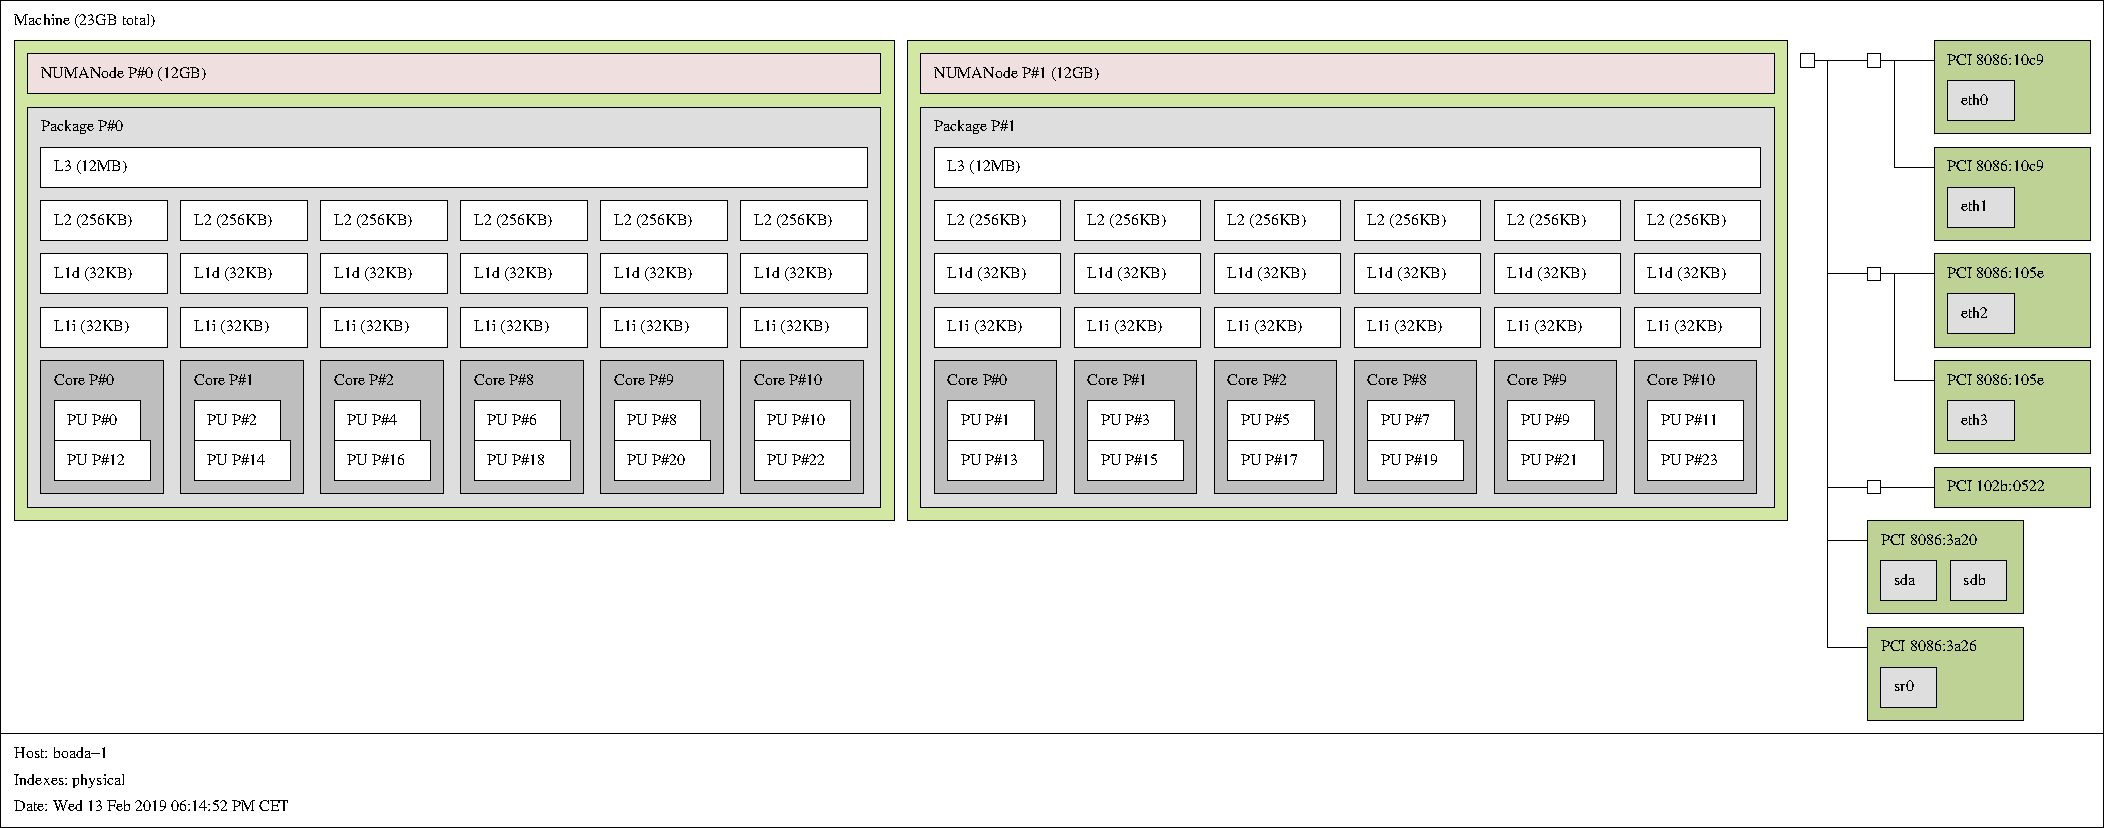
\includegraphics[scale=0.25]{./images/boada1-4}
  \caption{Architectural diagram for the node \textbf{boada-1}, obtained using the \textbf{lstopo} command.}
  \label{etiqueta}
\end{figure}

\subsection{Serial compilation and execution}

In this part, we have worked with a code used to find an approximation of the pi number.
We have used this code to test the performance of the executable in the different nodes of boada. There is a big difference executing the code in one node or in another. In node 1, it is executed interactively (since everyone is connected at the same time in this node) whereas in the other nodes, we will achieve an isolated execution ensuring the maximum performance of the node.
We have obtained the following results:\newline

Execution time in node 1: 3.939644 s

Execution time in node 4: 3.958794 s\newline

Theoretically the execution time in node 4 should be smaller than in node 1 but we have supposed that the status of the machine (maybe too heat) can cause this difference.

\subsection{Compilation and execution of OpenMP programs}

In this part of the laboratory we made the first contact with an OpenMP code, where we have been able to observe different instructions used to carry out with the parallelization.
Executing the code we have obtained the following results interactively in the node 1:\newline

Execution time with 1 thread: 3.944351 s

Execution time with 8 thread: 0.581683 s\newline

And then the same code has been executed isolated in the node 3:\newline

Execution time with 1 thread: 3.944042 s

Execution time with 8 thread: 0.943658 s\newline

As we can see, the execution in node 1 is again smaller than in node 3 for the same reason we said before.

\section{Strong vs. weak scalability}

In this section we had to explore the scalability of the parallel version in \textbf{pi\_omp.c}. This scalability is measured calculating the speedup. This is the ratio between the sequential and the parallel execution times. To do this, we had 2 different scenarios: \textit{Strong scalability} and \textit{Weak scalability}.

\subsection{Strong scalability}

Strong scalability is a technique where the number of threads is changed with a fixed problem size. In this case parallelism is used to reduce the execution time of the program.

We are going to compare the execution time of \textbf{pi\_omp.c} in the 3 different node architectures. We will see that is not always a good solution to increase the number of threads as much as we can, because it will appear a lot of overhead time.

\subsubsection{Boada 1-4}

As we can see in Figure \ref{fig:strong_v1_1} the execution time decreases as we increase the number of threads, reaching an optimum point in 11 threads. Then, it begins to increase again. This may be because of the overhead times when creating tasks, synchronizating and asking for data between them.

In the second figure, on the other hand, we can observe the real speedup (continuous line) and the teoric speedup (dashed line). The ideal case would be when the real speedup is coincident with the teoric speedup. This is not the case for the reason we said before (time overheads). We see a maximum speedup when the number of threads is 11. This is when the execution time is the minimum.

\begin{figure}[ht]
\begin{minipage}[b]{0.45\linewidth}
\centering
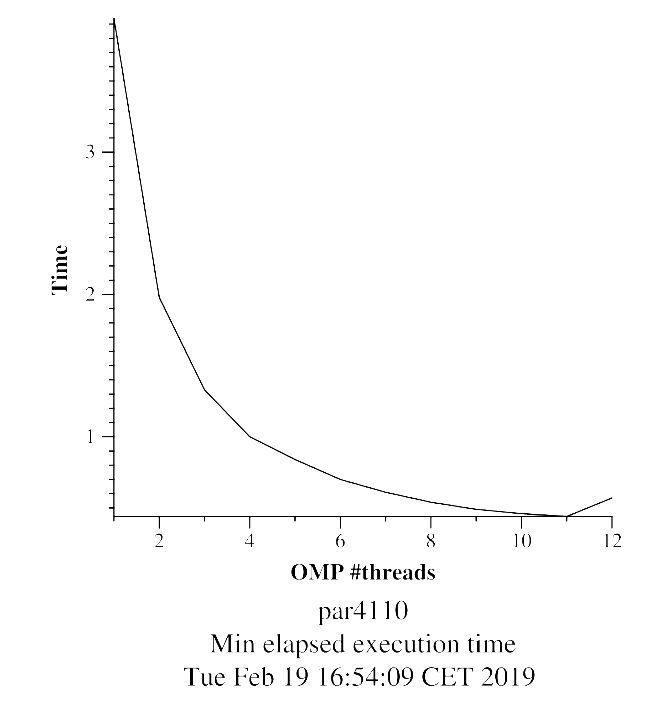
\includegraphics[width=\textwidth]{./images/strong_v1_1}
\caption{Execution time plot varying the number of threads in boada 1-4.}
\label{fig:strong_v1_1}
\end{minipage}
\hspace{0.5cm}
\begin{minipage}[b]{0.45\linewidth}
\centering
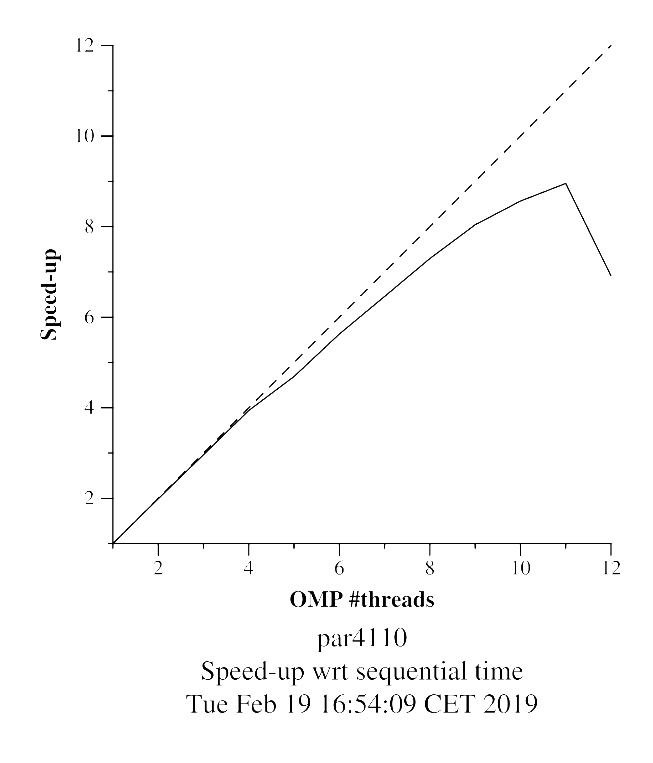
\includegraphics[width=\textwidth]{./images/strong_v1_2}

\caption{Speedup plot varying the number of threads in boada 1-4.}
\label{fig:strong_v1_2}
\end{minipage}
\end{figure}

\subsubsection{Boada 5}

We can see that Figure \ref{fig:strong_v5_1} is very similar than Figure \ref{fig:strong_v1_1} but with 12 threads it has not reached its minimum execution time. So we think that adding more threads would still decrease the time.

However, there is something rare in Figure \ref{fig:strong_v5_2}, because the real speedup is bigger than the teoric speedup, when the real speedup should never pass the teoric one. This means that the sequential version is faster than the parallel one. We discussed about it and we came to a conclusion: this happens because sequential code may have more hits in the cache than the parallel version, so it spends less time in memory accesses.

\begin{figure}[ht]
\begin{minipage}[b]{0.45\linewidth}
\centering
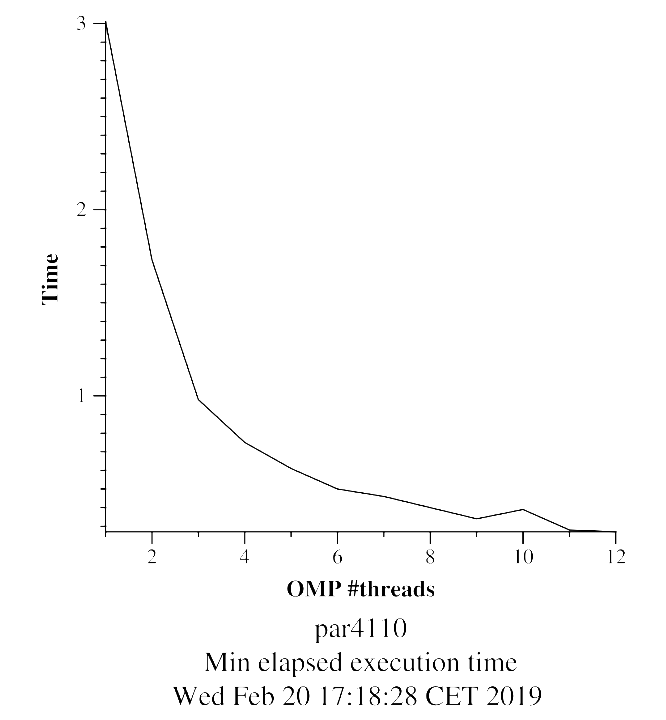
\includegraphics[width=\textwidth]{./images/strong_v5_1}
\caption{Execution time plot varying the number of threads in boada 5.}
\label{fig:strong_v5_1}
\end{minipage}
\hspace{0.5cm}
\begin{minipage}[b]{0.45\linewidth}
\centering
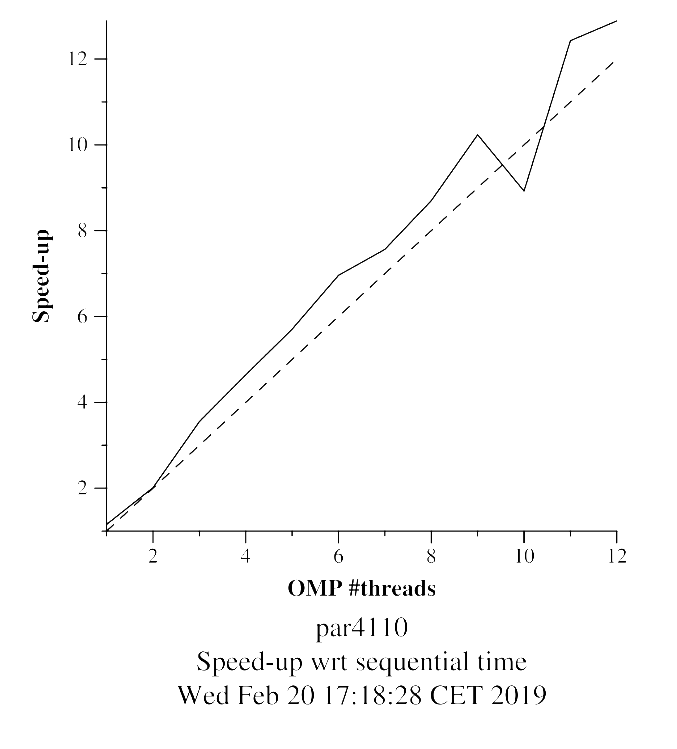
\includegraphics[width=\textwidth]{./images/strong_v5_2}

\caption{Speedup plot varying the number of threads in boada 5.}
\label{fig:strong_v5_2}
\end{minipage}
\end{figure}

\subsubsection{Boada 6-8}

In this point, all important things have been explained before. The only difference is that this architecture seems to be better than the rest, with a speedup that increases linear and is coincident with the teoric one. In this nodes there are also time overheads, but as it is a newer version, this overheads may be treated better. If we do the same plot using a bigger number of threads, the real speedup will decay for sure and will become a similar plot from the previous ones.

\begin{figure}[H]
\begin{minipage}[b]{0.45\linewidth}
\centering
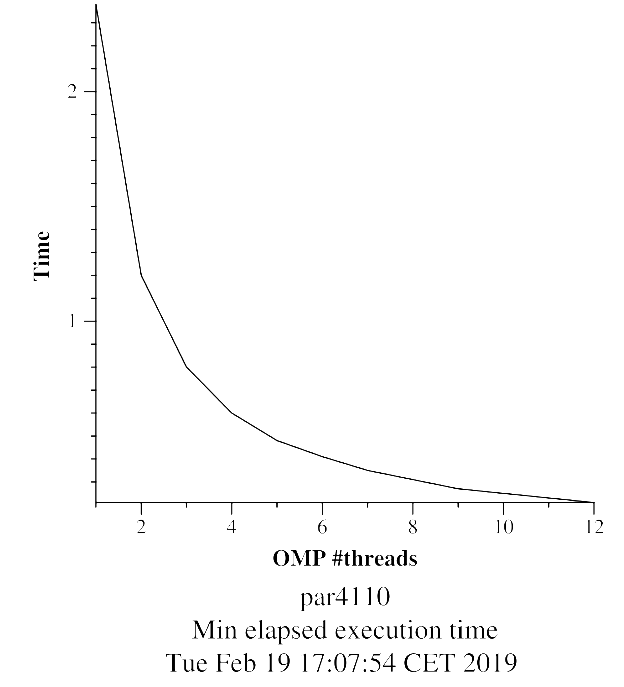
\includegraphics[width=\textwidth]{./images/strong_v7_1}
\caption{Execution time plot varying the number of threads in boada 6-8.}
\label{fig:strong_v7_1}
\end{minipage}
\hspace{0.5cm}
\begin{minipage}[b]{0.45\linewidth}
\centering
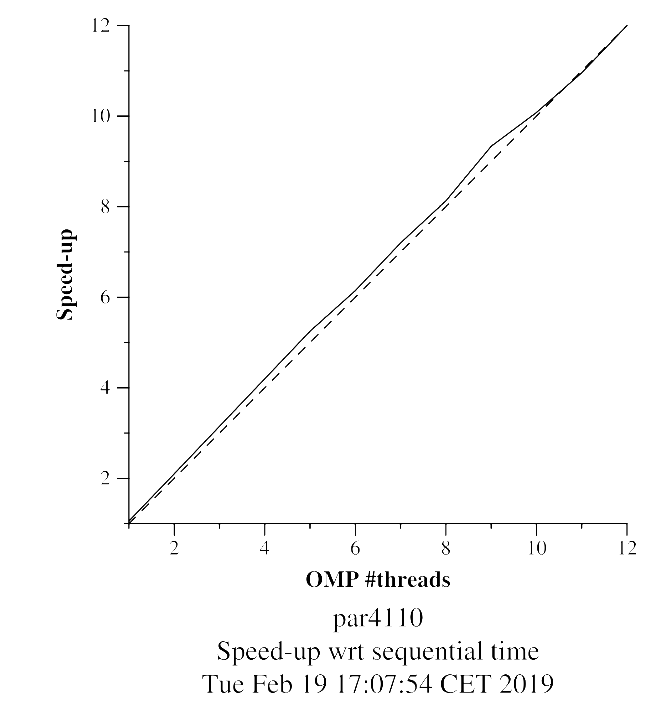
\includegraphics[width=\textwidth]{./images/strong_v7_2}

\caption{Speedup plot varying the number of threads in boada 6-8.}
\label{fig:strong_v7_2}
\end{minipage}
\end{figure}

To conclude, boada 6-8 seems to be the best architecture of the 3 we have in strong scalability because it is the one where the real speedup is more time coincident with the teoric speedup.

\subsection{Weak scalability}

In weak scalability, the problem size is proportional to the number of threads. In this case parallelism is used to increase the problem size for which the program is executed.

\subsubsection{Boada 1-4}

In Figure \ref{fig:weak_v1}, the teoric speedup would be a horizontal line in $y = 1.0$ but this does not happen for the reason we said before, the overhead times. The abrupt decrease is found from 9 to 11 threads, when t$_{create}$, t$_{sync}$ and t$_{access}$ begin to be relevant in the execution time.

%\begin{figure}[H]
%  \centering
%  \includegraphics[scale=0.65]{./lab1/pi/weak_v1}
%  \caption{Pie de figura}
%  \label{weak_v1}
%\end{figure}

\subsubsection{Boada 5}

In Figure \ref{fig:weak_v5} we can observe again that the real speedup is greater than the teoric speedup due to cache hits and misses, as we said in the previous section.

%\begin{figure}[H]
%  \centering
%  \includegraphics[scale=0.65]{./lab1/pi/weak_v5}
%  \caption{Pie de figura}
%  \label{weak_v5}
%\end{figure}

\subsubsection{Boada 6-8}

Finally, in boada 6-8 we see that the speedup stays quite good with respect to the teoric one. It only decreases at the begining. Then, it stays constant in $y \approx 0.96$, which is very good.

\begin{figure}[ht]
\begin{minipage}[b]{0.30\linewidth}
\centering
\includegraphics[width=\textwidth]{./images/weak_v1}
\caption{Execution time plot varying the number of threads and the problem size in boada 1-4.}
\label{fig:weak_v1}
\end{minipage}
\hspace{0.5cm}
\begin{minipage}[b]{0.30\linewidth}
\centering
\includegraphics[width=\textwidth]{./images/weak_v5}

\caption{Execution time plot varying the number of threads and the problem size in boada 5.}
\label{fig:weak_v5}
\end{minipage}
\hspace{0.5cm}
\begin{minipage}[b]{0.30\linewidth}
\centering
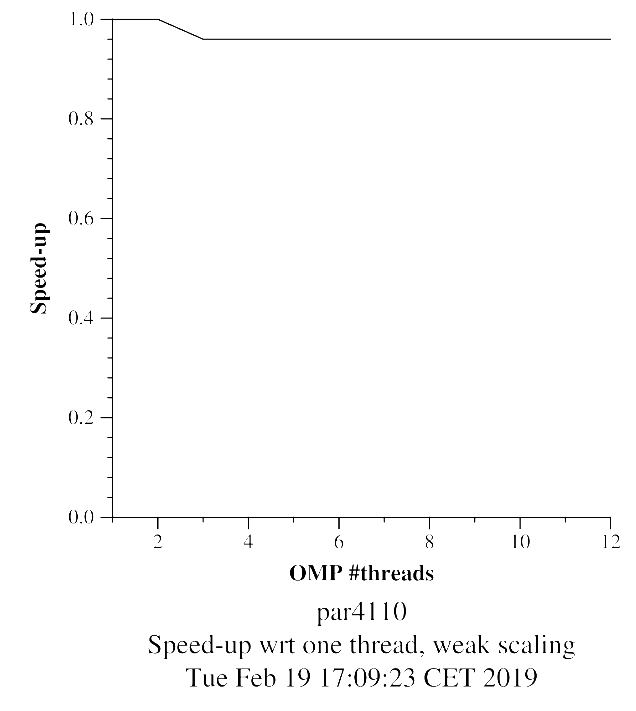
\includegraphics[width=\textwidth]{./images/weak_v8}

\caption{Execution time plot varying the number of threads and the problem size in boada 6-8.}
\label{fig:weak_v8}
\end{minipage}
\end{figure}

Again, we can conclude that boada 6-8 architecture is the best solution in weak scalability.

\section{Analysis of task decompositions for 3DFFT}

In order to do the analysis we have used \textit{Tareador}, which helped us to see the task dependence graph and analyse  the variables whose access provokes each data dependence between a pair of nodes (tasks). Moreover we have also used \textit{Paraver} that showed the timeline for the simulated execution using the number of processors that we wanted. Even though the maximum number of processors that \textit{Paraver} could simulate was 128, we never had to use all of them to get the maximum parallelism of the code. However, it was useful to know what the T$_\infty$ was.

\subsection{Original Version}

In this version, there were few parts of the code parallelised, so parallelism will be small.

To do the calculations manually, we need the time of execution per instruction. To do this, we need the total number of instructions and the T$_1$. Afterwards, we only have to divide the number of instructions by the T$_1$. Thus, T$_{instruction}$ = 639780001/639780 $\approx$ 1000 ns.

Using T$_{instruction}$ we can now calculate the data we want. On the one hand, T$_1$ refers to the execution time of the code in sequential mode (using only 1 processor). Hence, we have to multiply T$_{instruction}$ by the total number of instructions. On the other hand, T$_\infty$ refers to the execution time of the code when we have an infinite number of processors. T$_\infty$ is calculated finding the critical path in the task dependency graph. This is the largest path that cannot be parallelised. Then, we multiply the number of instructions in the critical path by T$_{instruction}$.

\[T_1 = 639780 * 1000 = 639780000  ns \]
\[T_\infty = 639760 * 1000 = 639760000  ns \]

As we can see, T$_1$ and T$_\infty$ values are very similar from the ones of the \textit{Tareador}.

Finally, we had to compute the Parallelism, which refers to how fast would we go if sufficient (infinite) resources were available. For computing it we divided T$_1$ by T$_\infty$.

\[ Parallelism = 639780000/639760000 = 1.00003126172 \]

The following code is the one extracted from the original version. We can easily see that this code can be decomposed into finer\textendash gained tasks. We will see how we decompose it in the following versions. Figure \ref{dependency_graph_base} reflects the need we have to decompose the tasks to reduce the execution time and increase the parallelism, as task \textit{init\_complex\_grid} (red task) has 100442 instructions and \textit{ffts1\_and\_transpositions} (yellow task) has 539208 instructions.

\begin{lstlisting}
	START_COUNT_TIME;
	
	tareador_start_task("Seq code");
	
	ffts1_planes(p1d, in_fftw);
	transpose_xy_planes(tmp_fftw, in_fftw);
	ffts1_planes(p1d, tmp_fftw);
	transpose_zx_planes(in_fftw, tmp_fftw);
	ffts1_planes(p1d, in_fftw);
	transpose_zx_planes(tmp_fftw, in_fftw);
	transpose_xy_planes(in_fftw, tmp_fftw);
	
	tareador_edn_task("Seq code");
	
	STOP_COUNT_TIME("Execution FFT3D");
	
	...
\end{lstlisting}

\begin{figure}[H]
  \centering
  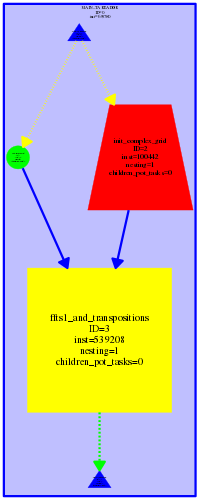
\includegraphics{./images/dependency_graph_base}
  \caption{Task dependecy graph of the original version.}
  \label{dependency_graph_base}
\end{figure}

\subsection{Version 1}

From now on, we are not going to talk again on how to compute T$_\infty$ and Parallelism because it is the same explained in the previous section. Moreover, T$_{instruction}$ and T$_1$ will remain the same values due to the fact that we are executing the code in the same boada node and the code lines are always the same.

\[ T_\infty = (110 + 100442 + 103144 + 57444 + 103144 + 57444 + 103144 + 57444 + 57444 + 0) * 1000 \]
\[ =  639760 * 1000 = 639760000 ns \]


\[ Parallelism = T_1/T_\infty = 639780000/639760000 = 1.000031262 \]

In this first version of the code we created one task for each function that was inside the "big" task of the original code. As a consequence, the work that was doing just one processor could now be done by 7 processors at the same time. This is not true because of the dependencies that are created. This can be seen in Figure \ref{dependency_graph_v1}. The yellow task cannot be executed until the red and green ones end, the purple task cannot be executed until the yellow task terminates, and so on. For this reason, the Parallelism is approximately 1 because, even though we have decomposed the tasks, only 1 big task can be executed at the same time, altough we have had an infinite number of processors.

\begin{lstlisting}
    START_COUNT_TIME;

    tareador_start_task("ffts1_and_transpositions_1");
        ffts1_planes(p1d, in_fftw);
    tareador_end_task("ffts1_and_transpositions_1");

    tareador_start_task("ffts1_and_transpositions_2");
        transpose_xy_planes(tmp_fftw, in_fftw);
    tareador_end_task("ffts1_and_transpositions_2");

    tareador_start_task("ffts1_and_transpositions_3");
        ffts1_planes(p1d, tmp_fftw);
    tareador_end_task("ffts1_and_transpositions_3");

    tareador_start_task("ffts1_and_transpositions_4");
        transpose_zx_planes(in_fftw, tmp_fftw);
    tareador_end_task("ffts1_and_transpositions_4");

    tareador_start_task("ffts1_and_transpositions_5");
        ffts1_planes(p1d, in_fftw);
    tareador_end_task("ffts1_and_transpositions_5");

    tareador_start_task("ffts1_and_transpositions_6");
        transpose_zx_planes(tmp_fftw, in_fftw);
    tareador_end_task("ffts1_and_transpositions_6");

    tareador_start_task("ffts1_and_transpositions_7");
        transpose_xy_planes(in_fftw, tmp_fftw);
    tareador_end_task("ffts1_and_transpositions_7");
     
    STOP_COUNT_TIME("Execution FFT3D");
    
    ...
\end{lstlisting}

\begin{figure}[H]
  \centering
  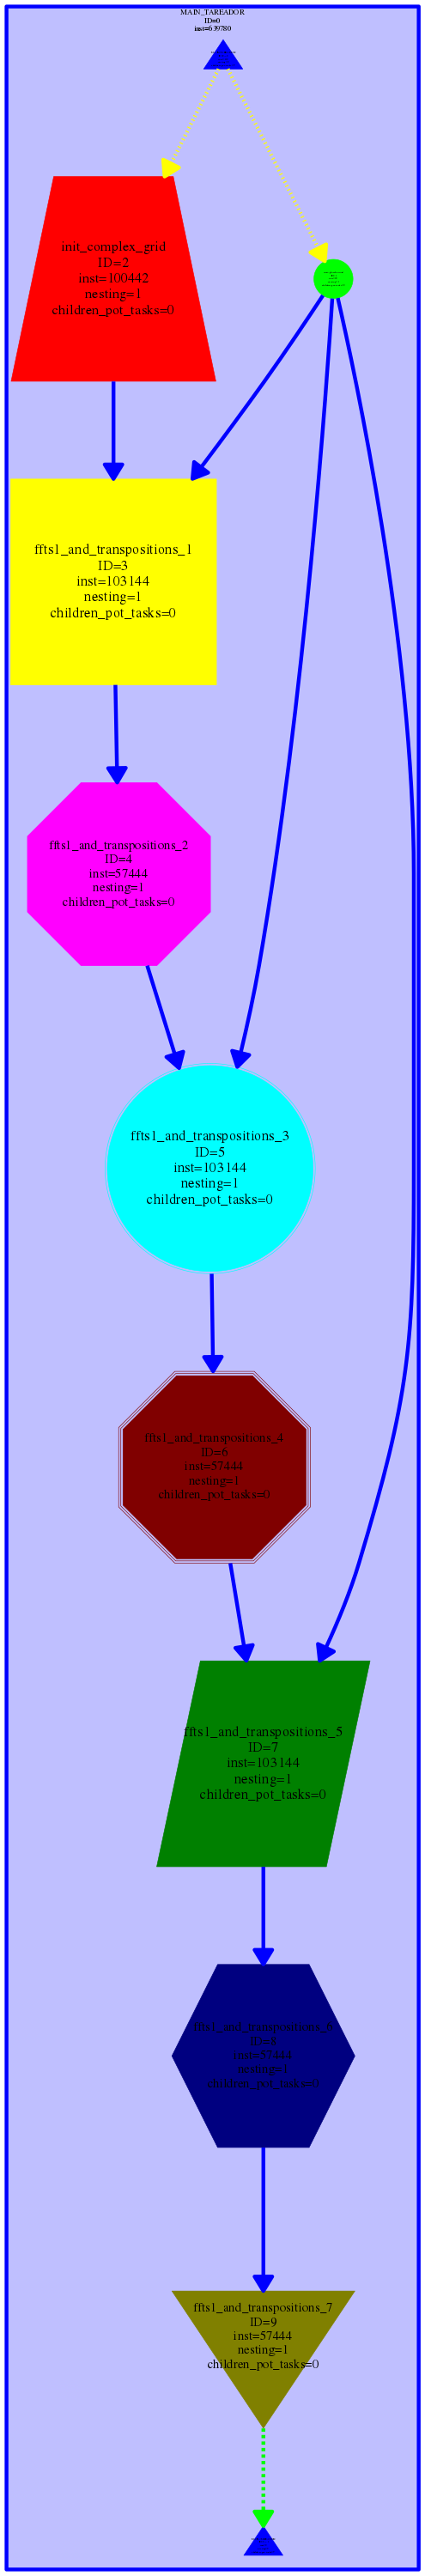
\includegraphics[width=5cm,height=20cm]{./images/dependency_graph_v1}
  \caption{Task dependency graph of version 1.}
  \label{dependency_graph_v1}
\end{figure}

\subsection{Version 2}

We have seen in version 1 that creating a task each time we call a function is not a good decision at all due to the dependencies. However, if we create the tasks inside the first for of some functions, we will be able to parallelise more the code because for every iteration of the loop we will create another task that can be executed in a different processor.

In this version, we will only modify the function \textit{ffts1\_planes}. We will create one task for every iteration of the most outer loop of the function. Thus, we will create N different tasks every time we call this function. The code below shows how we have done it.

\[ T_\infty = (57 + 100442 + 10305 + 57444 + 10305 + 57444 + 10305 + 57444 + 57444 + 0) * 1000\]

\[ = 361190 * 1000 = 361190000 ns \]

\[ Parallelism = T_1/T_\infty = 639780000/361190000 = 1.771311498 \]

We can see that now the parallelism has increased a lot in comparison to the one in version 1 and the critical path has decreased a lot.

\begin{lstlisting}
	void ffts1_planes(fftwf_plan p1d, fftwf_complex in_fftw[][N][N]) {
	    int k,j;
	
	    for (k=0; k<N; k++) {
	     tareador_start_task("ffts1_planes_loop_k");
	     for (j=0; j<N; j++) {
	       fftwf_execute_dft( p1d, (fftwf_complex *)in_fftw[k][j][0],
	       					(fftwf_complex *)in_fftw[k][j][0]);
	     }
	     tareador_end_task("ffts1_planes_loop_k");
	
	    }
	}

	...

	int main(){
	
		...
	
		START_COUNT_TIME;
	
	    ffts1_planes(p1d, in_fftw);
	
	    tareador_start_task("ffts1_and_transpositions_2");
	        transpose_xy_planes(tmp_fftw, in_fftw);
	    tareador_end_task("ffts1_and_transpositions_2");
	
	    ffts1_planes(p1d, tmp_fftw);
	
	    tareador_start_task("ffts1_and_transpositions_4");
	        transpose_zx_planes(in_fftw, tmp_fftw);
	    tareador_end_task("ffts1_and_transpositions_4");
	
	    ffts1_planes(p1d, in_fftw);
	
	    tareador_start_task("ffts1_and_transpositions_6");
	        transpose_zx_planes(tmp_fftw, in_fftw);
	    tareador_end_task("ffts1_and_transpositions_6");
	
	    tareador_start_task("ffts1_and_transpositions_7");
	        transpose_xy_planes(in_fftw, tmp_fftw);
	    tareador_end_task("ffts1_and_transpositions_7");
	     
    	STOP_COUNT_TIME("Execution FFT3D");
    	
    	...
    }
\end{lstlisting}

In Figure \ref{dependency_graph_v2} we can see that the yellow task of Figure \ref{dependency_graph_v1} has been decomposed into smaller tasks (the yellow ones too). Now, up to 10 processors can execute these diferent tasks at the same time, because there is no dependencies between them.

\begin{figure}[H]
  \centering
  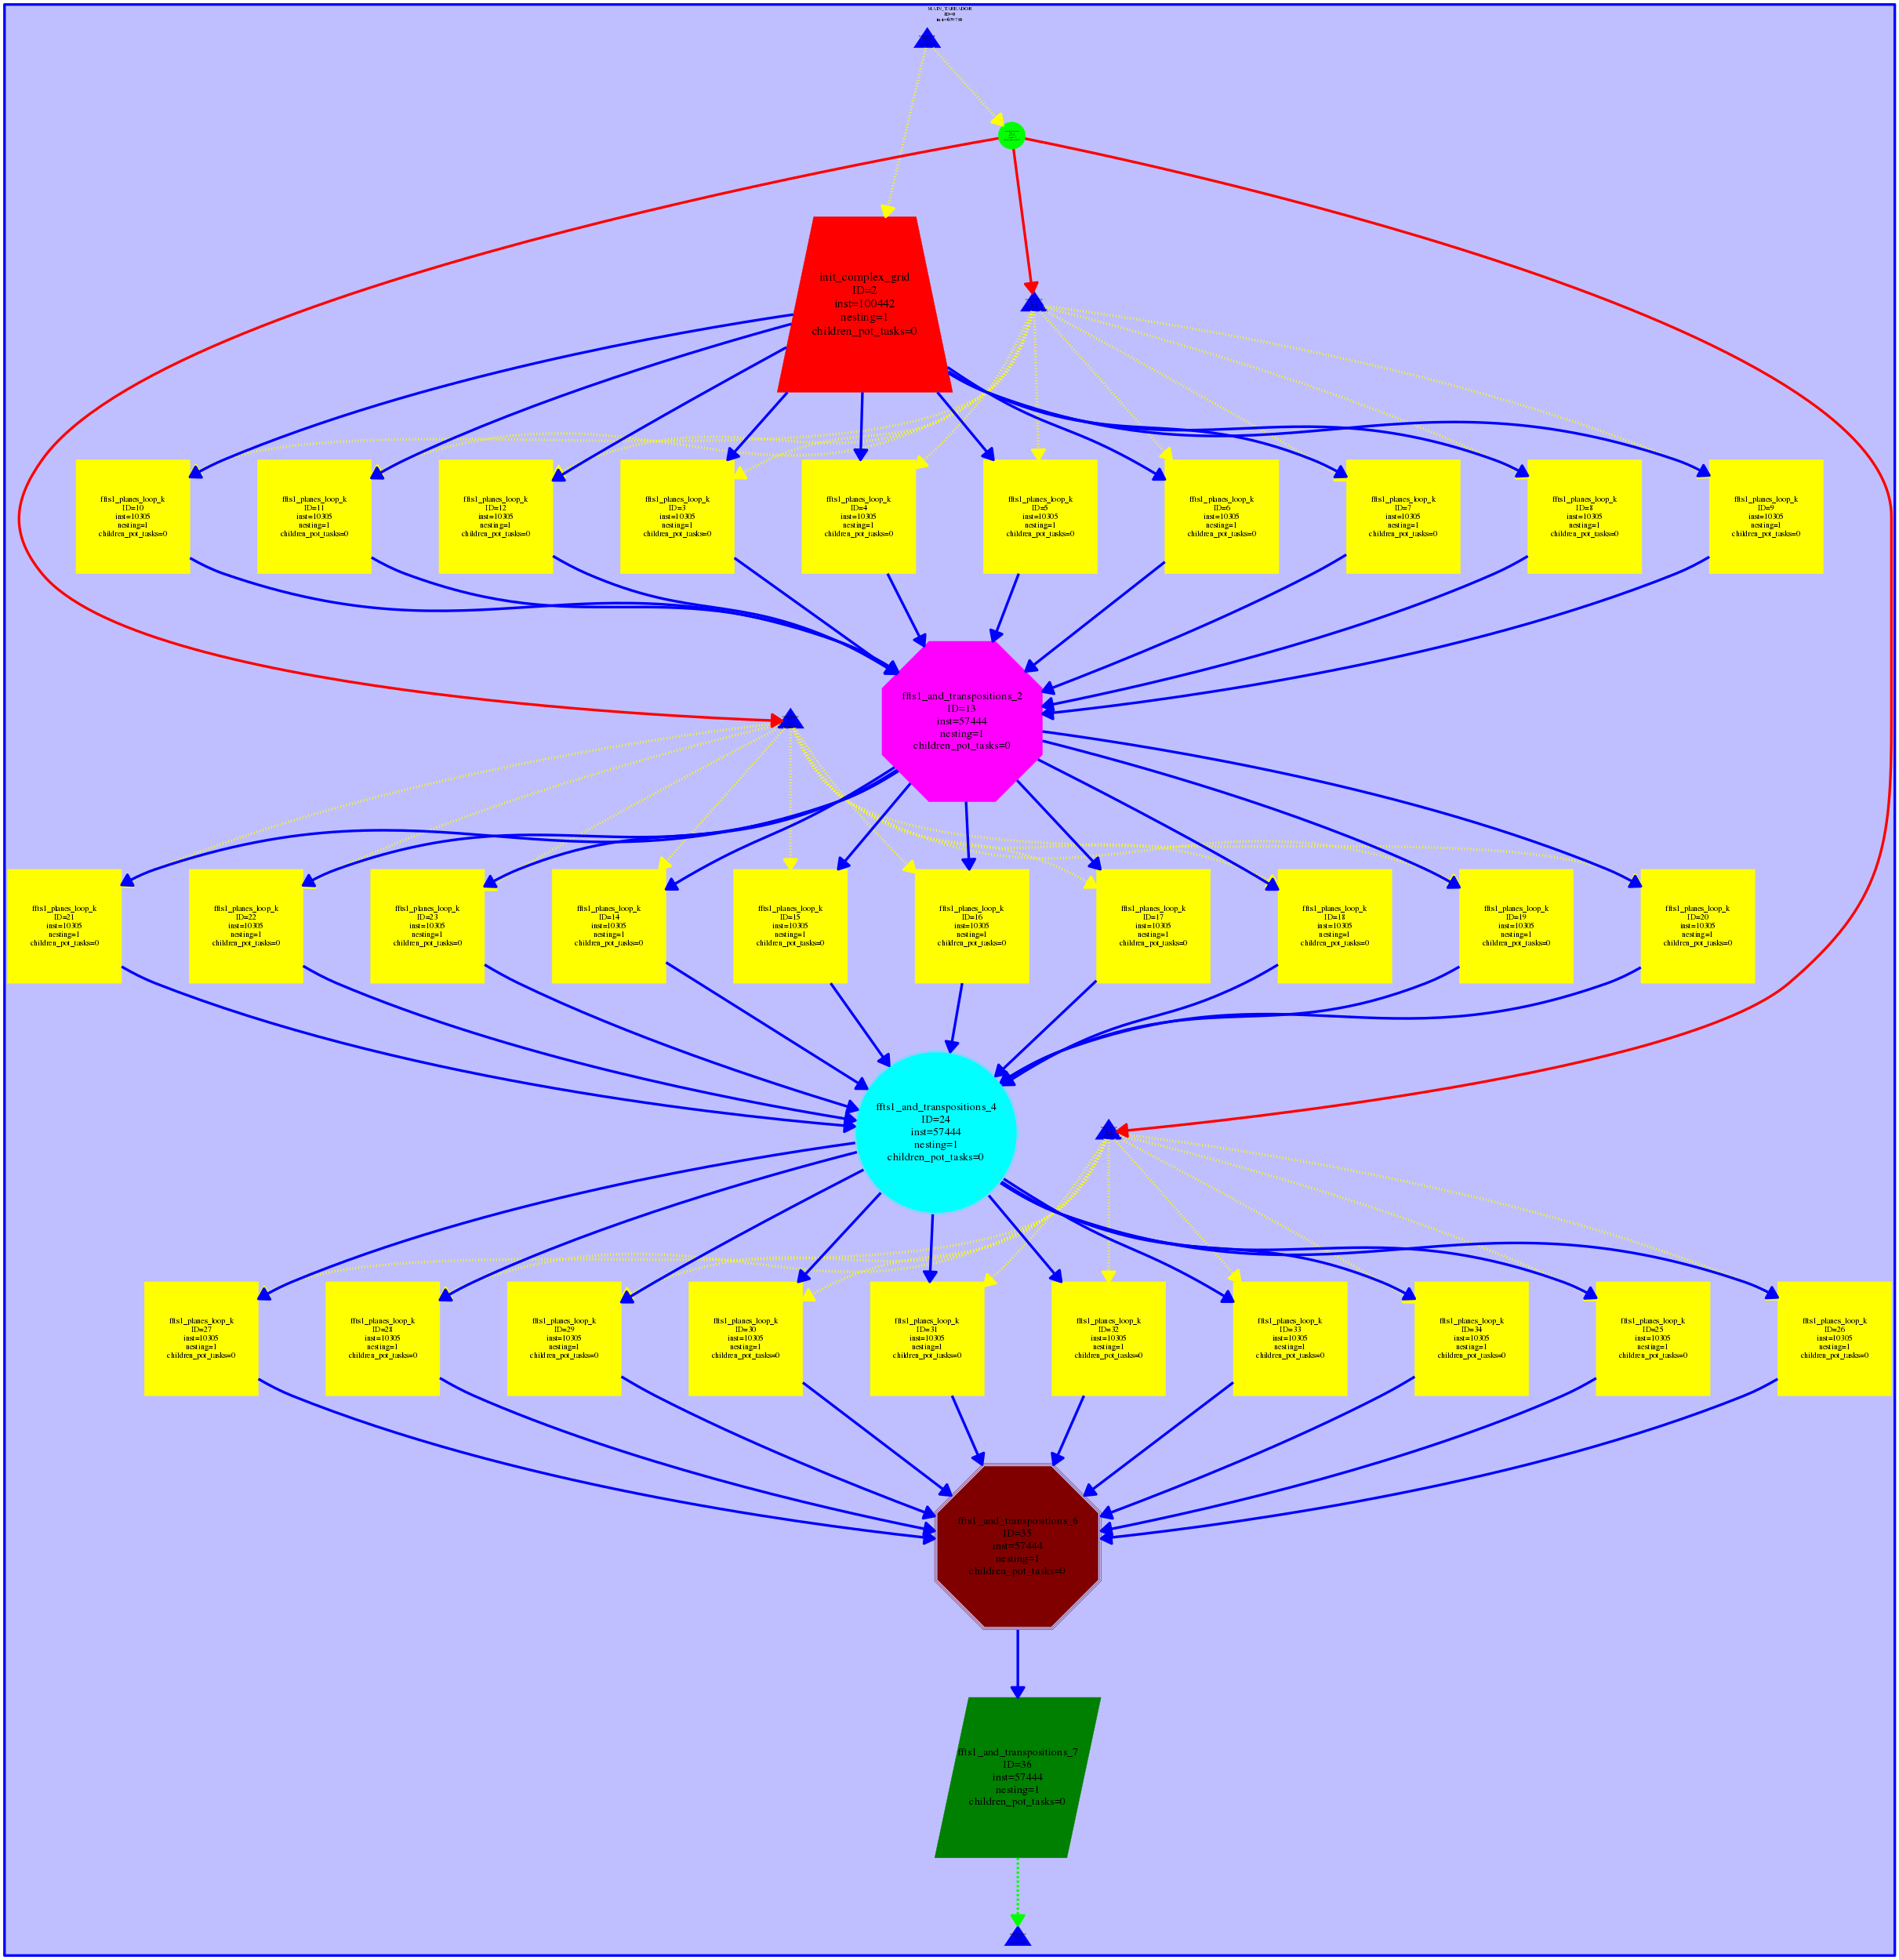
\includegraphics[width=15cm,height=15cm]{./images/dependency_graph_v2}
  \caption{Task dependency graph of version 2.}
  \label{dependency_graph_v2}
\end{figure}


\subsection{Version 3}

As we saw that the modification in version 2 improved the parallelism and decreased T$_\infty$, we continued "on the same line", so we started modifying \textit{transpose\_xy\_planes} and \textit{transpose\_zx\_planes} using the same strategy than in version 2. This is creating the tasks inside the functions, specifically inside the most outer loop. Doing this we got the following results:

\[ T_\infty = (57 + 100442 + 10305 + 5735 + 10305 + 5735 + 10305 + 5735 + 5375 + 0) * 1000 \]

\[ = 154354 * 1000 = 154354000 ns \]

\[ Parallelism = T_1/T_\infty = 639780000/154354000 = 4.144887726 \]

In this version, Parallelism has increased much more than in version 2. In Figure \ref{dependency_graph_v3} we can see that the purple and light blue tasks of Figure \ref{dependency_graph_v2} have now become 10 tasks respectively (these 2 loop also depend on the N value).

\begin{lstlisting}
void transpose_xy_planes(fftwf_complex  tmp_fftw[][N][N],
						 fftwf_complex in_fftw[][N][N]) {
	    int k,j,i;
	
	    for (k=0; k<N; k++) {
	     tareador_start_task("ffts1_transpose_xy_loop_k");
	     for (j=0; j<N; j++) {
	       for (i=0; i<N; i++)
	       {
	         tmp_fftw[k][i][j][0] = in_fftw[k][j][i][0];
	         tmp_fftw[k][i][j][1] = in_fftw[k][j][i][1];
	       }
	     }
	     tareador_end_task("ffts1_transpose_xy_loop_k");
	    }
	}
	
	void transpose_zx_planes(fftwf_complex in_fftw[][N][N],
							 fftwf_complex tmp_fftw[][N][N]) {
	    int k, j, i;
	
	    for (k=0; k<N; k++) {
	     tareador_start_task("ffts1_transpose_zx_loop_k");
	     for (j=0; j<N; j++) {
	       for (i=0; i<N; i++)
	       {
	         in_fftw[i][j][k][0] = tmp_fftw[k][j][i][0];
	         in_fftw[i][j][k][1] = tmp_fftw[k][j][i][1];
	       }
	     }
	     tareador_end_task("ffts1_transpose_zx_loop_k");
	    }
	}
	
	...
	
	int main() {
	
		...	
		
	    START_COUNT_TIME;
	    
	    tareador_start_task("init_complex_grid");
	    init_complex_grid(in_fftw);
	    tareador_end_task("init_complex_grid");
	
	    STOP_COUNT_TIME("Init Complex Grid FFT3D");
	
	
	    START_COUNT_TIME;
	
	    ffts1_planes(p1d, in_fftw);
	    transpose_xy_planes(tmp_fftw, in_fftw);
	    ffts1_planes(p1d, tmp_fftw);
	    transpose_zx_planes(in_fftw, tmp_fftw);
	    ffts1_planes(p1d, in_fftw);
	    transpose_zx_planes(tmp_fftw, in_fftw);
	    transpose_xy_planes(in_fftw, tmp_fftw);
	     
	    STOP_COUNT_TIME("Execution FFT3D");
	    
	    ...
	}
\end{lstlisting}

\begin{figure}[H]
  \centering
  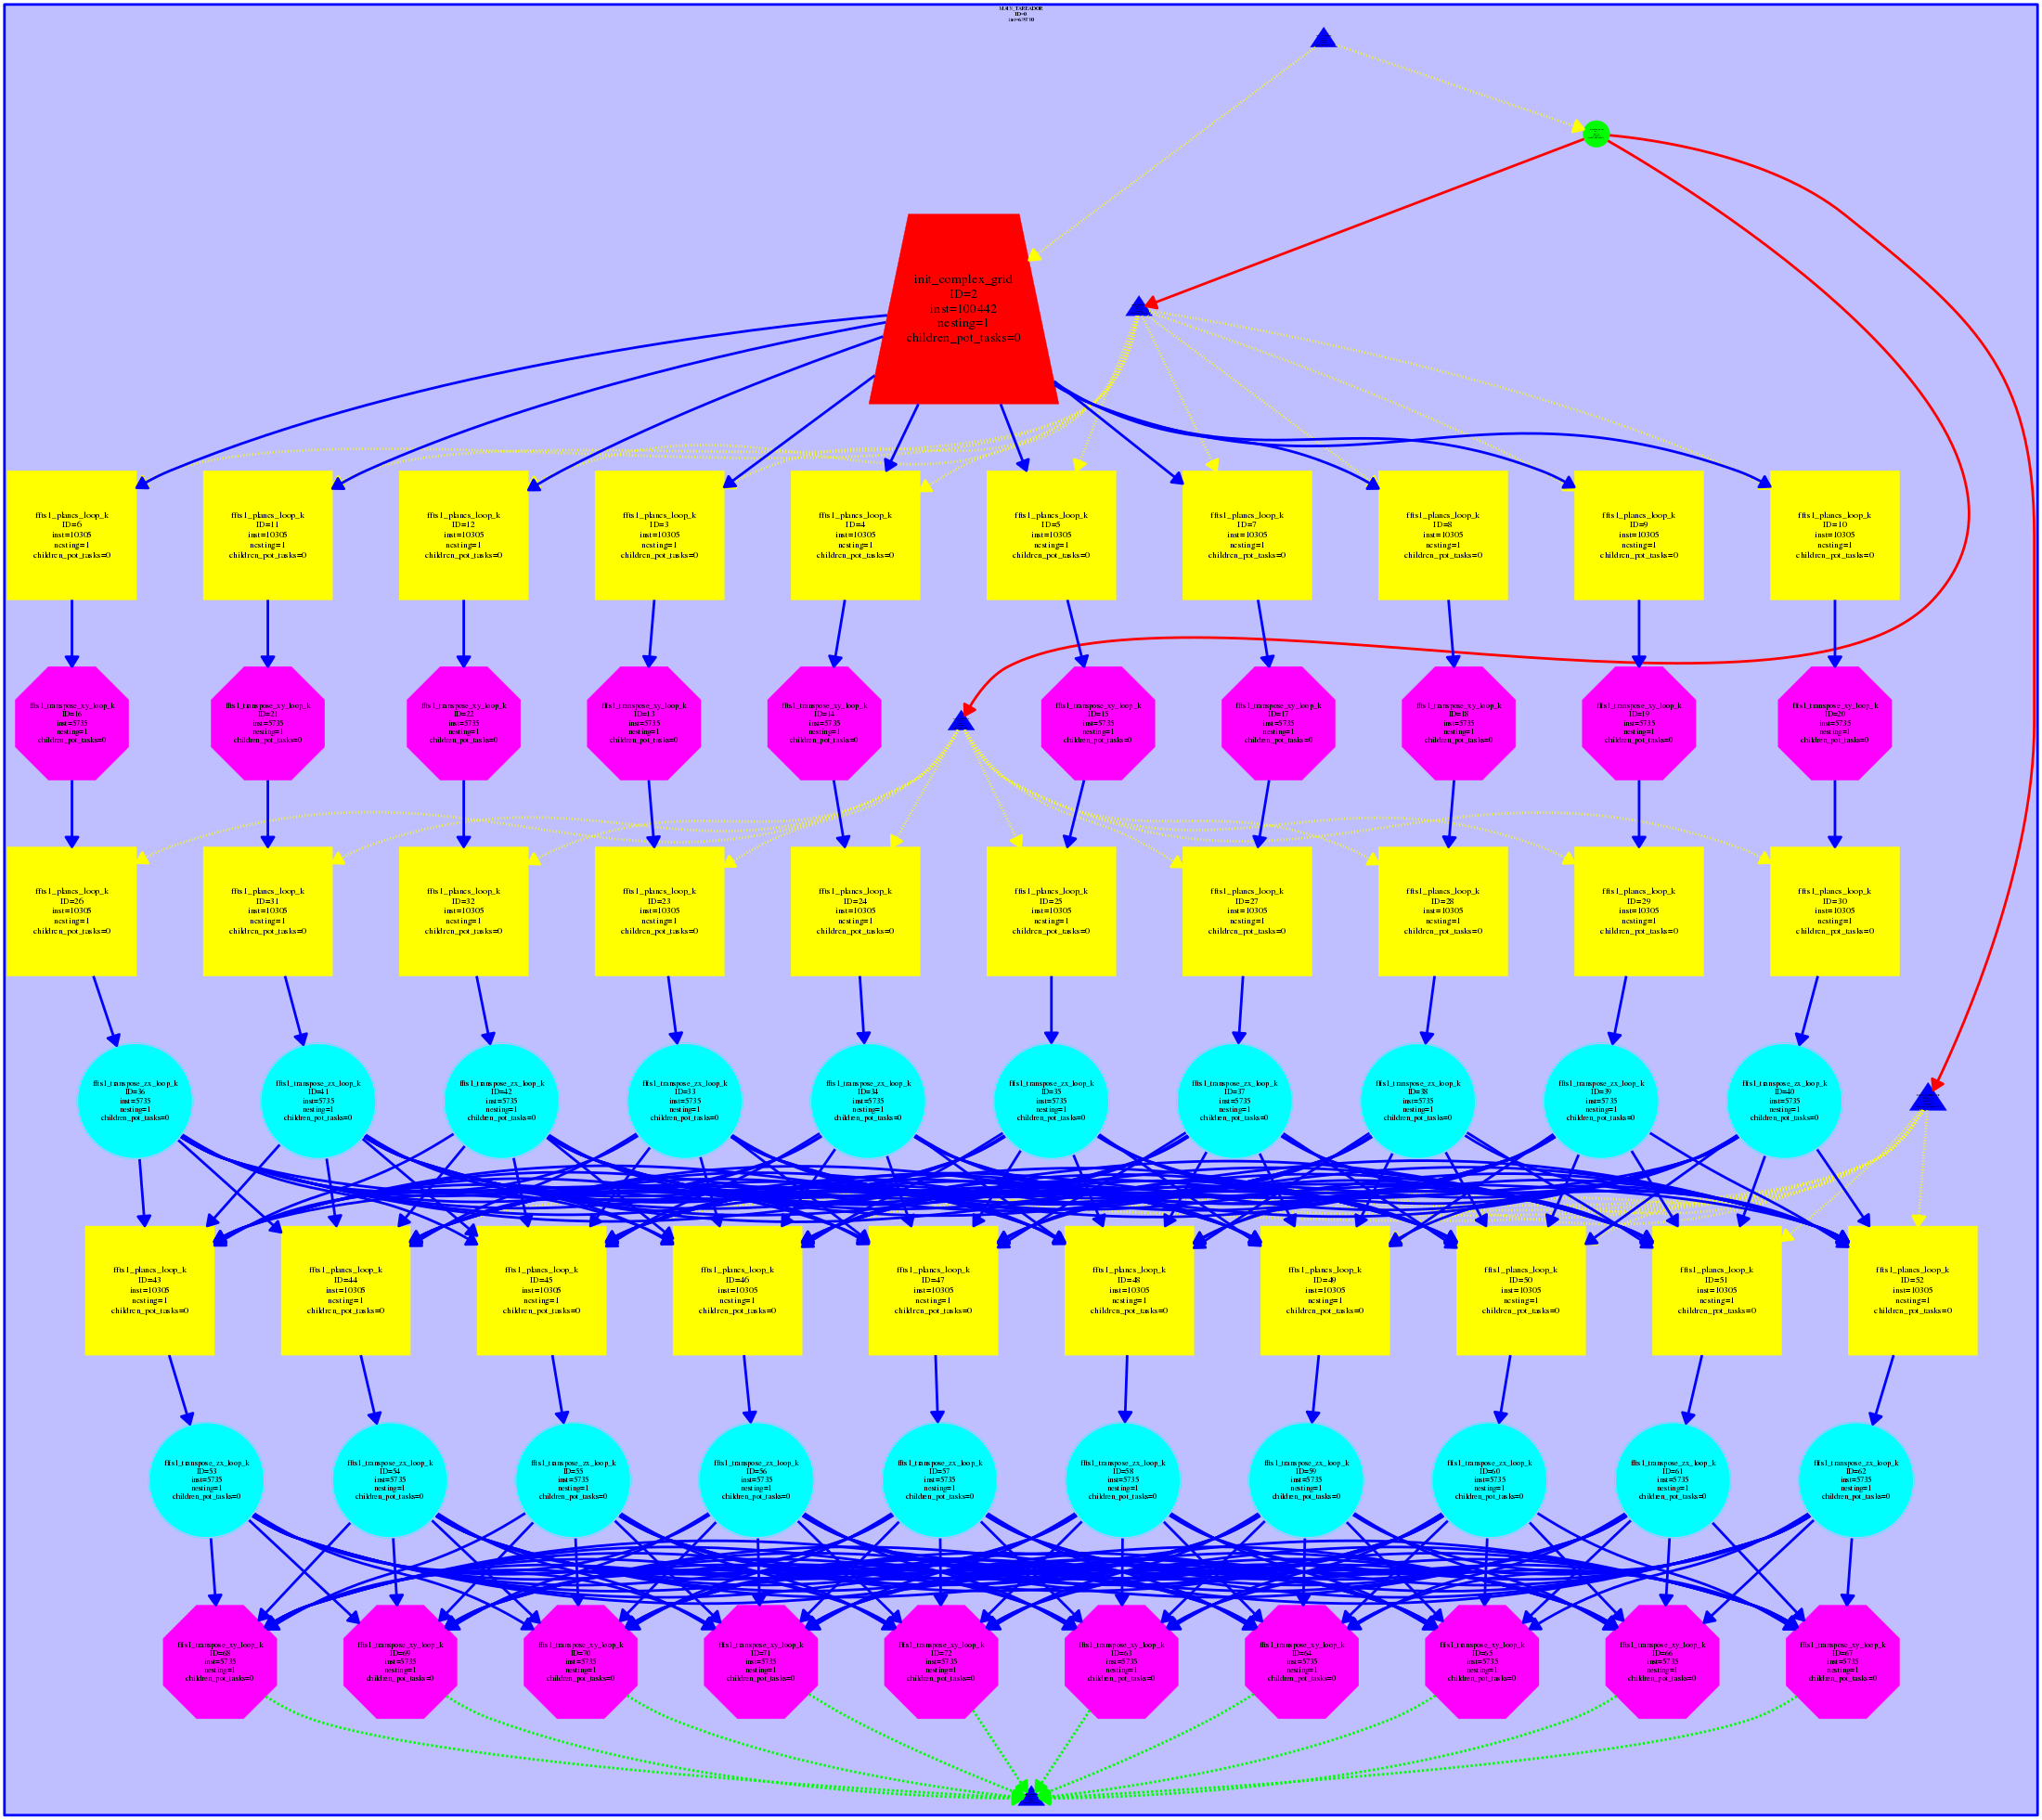
\includegraphics[width=15cm,height=13cm]{./images/dependency_graph_v3}
  \caption{Task dependency graph of version 3.}
  \label{dependency_graph_v3}
\end{figure}

\subsection{Version 4}

Even though in version 3 we improved a lot the code, in the previous figure we can see that there is still one task, the red one, that has 100442 instructions inside him, so we can also decompose this task into smaller ones doing the same modifications than the previous 2 versions.

We have modified the \textit{init\_complex\_grid} function, creating a new task every time we iterate through the most outer loop of the function. We can see the modifications graphically in Figure \ref{dependency_graph_v4} (red tasks). Again, there are N new tasks.

\[ T_\infty = (128 + 10035 + 10305 + 5735 + 10305 + 5735 + 10305 + 5735 + 5375 + 0) * 1000 \]

\[  = 64018 * 1000 = 64018000 ns \]

\[ Parallelism = T_1/T_\infty = 639780000/64018000 = 9.993751757 \]

In this version, the parallelism has increased a lot with respect to version 3.

We also had to simulate this version of the code with 1, 2, 4, 8, 16 and 32 processors to analyse the potential strong scalability. This is discussed in the section \ref{Analysis of the potential strong scalability in v4 and v5}.

\begin{lstlisting}
	void init_complex_grid(fftwf_complex in_fftw[][N][N]) {
	  int k,j,i;
	
	  for (k = 0; k < N; k++) {
	    tareador_start_task("ffts1_complex_loop_k");
	    for (j = 0; j < N; j++) {
	      for (i = 0; i < N; i++)
	      {
	        in_fftw[k][j][i][0] = (float) (sin(M_PI*((float)i)/64.0)+
	        							   sin(M_PI*((float)i)/32.0)+
	        							   sin(M_PI*((float)i/16.0)));
	        in_fftw[k][j][i][1] = 0;
	#if TEST
	        out_fftw[k][j][i][0]= in_fftw[k][j][i][0];
	        out_fftw[k][j][i][1]= in_fftw[k][j][i][1];
	#endif
	      }
	    }
	    tareador_end_task("ffts1_complex_loop_k");
	  }
	}
	
	...
	
	int main() {
	
		...
		
		START_COUNT_TIME;
	
	    tareador_start_task("start_plan_forward");
	    start_plan_forward(in_fftw, &p1d);
	    tareador_end_task("start_plan_forward");
	
	    STOP_COUNT_TIME("3D FFT Plan Generation");
	
	
	    START_COUNT_TIME;
	
	    init_complex_grid(in_fftw);
	
	    STOP_COUNT_TIME("Init Complex Grid FFT3D");
	
	
	    START_COUNT_TIME;
	
	    ffts1_planes(p1d, in_fftw);
	    transpose_xy_planes(tmp_fftw, in_fftw);
	    ffts1_planes(p1d, tmp_fftw);
	    transpose_zx_planes(in_fftw, tmp_fftw);
	    ffts1_planes(p1d, in_fftw);
	    transpose_zx_planes(tmp_fftw, in_fftw);
	    transpose_xy_planes(in_fftw, tmp_fftw);
	     
	    STOP_COUNT_TIME("Execution FFT3D");
	    
	    ...
	}
\end{lstlisting}

\begin{figure}[H]
  \centering
  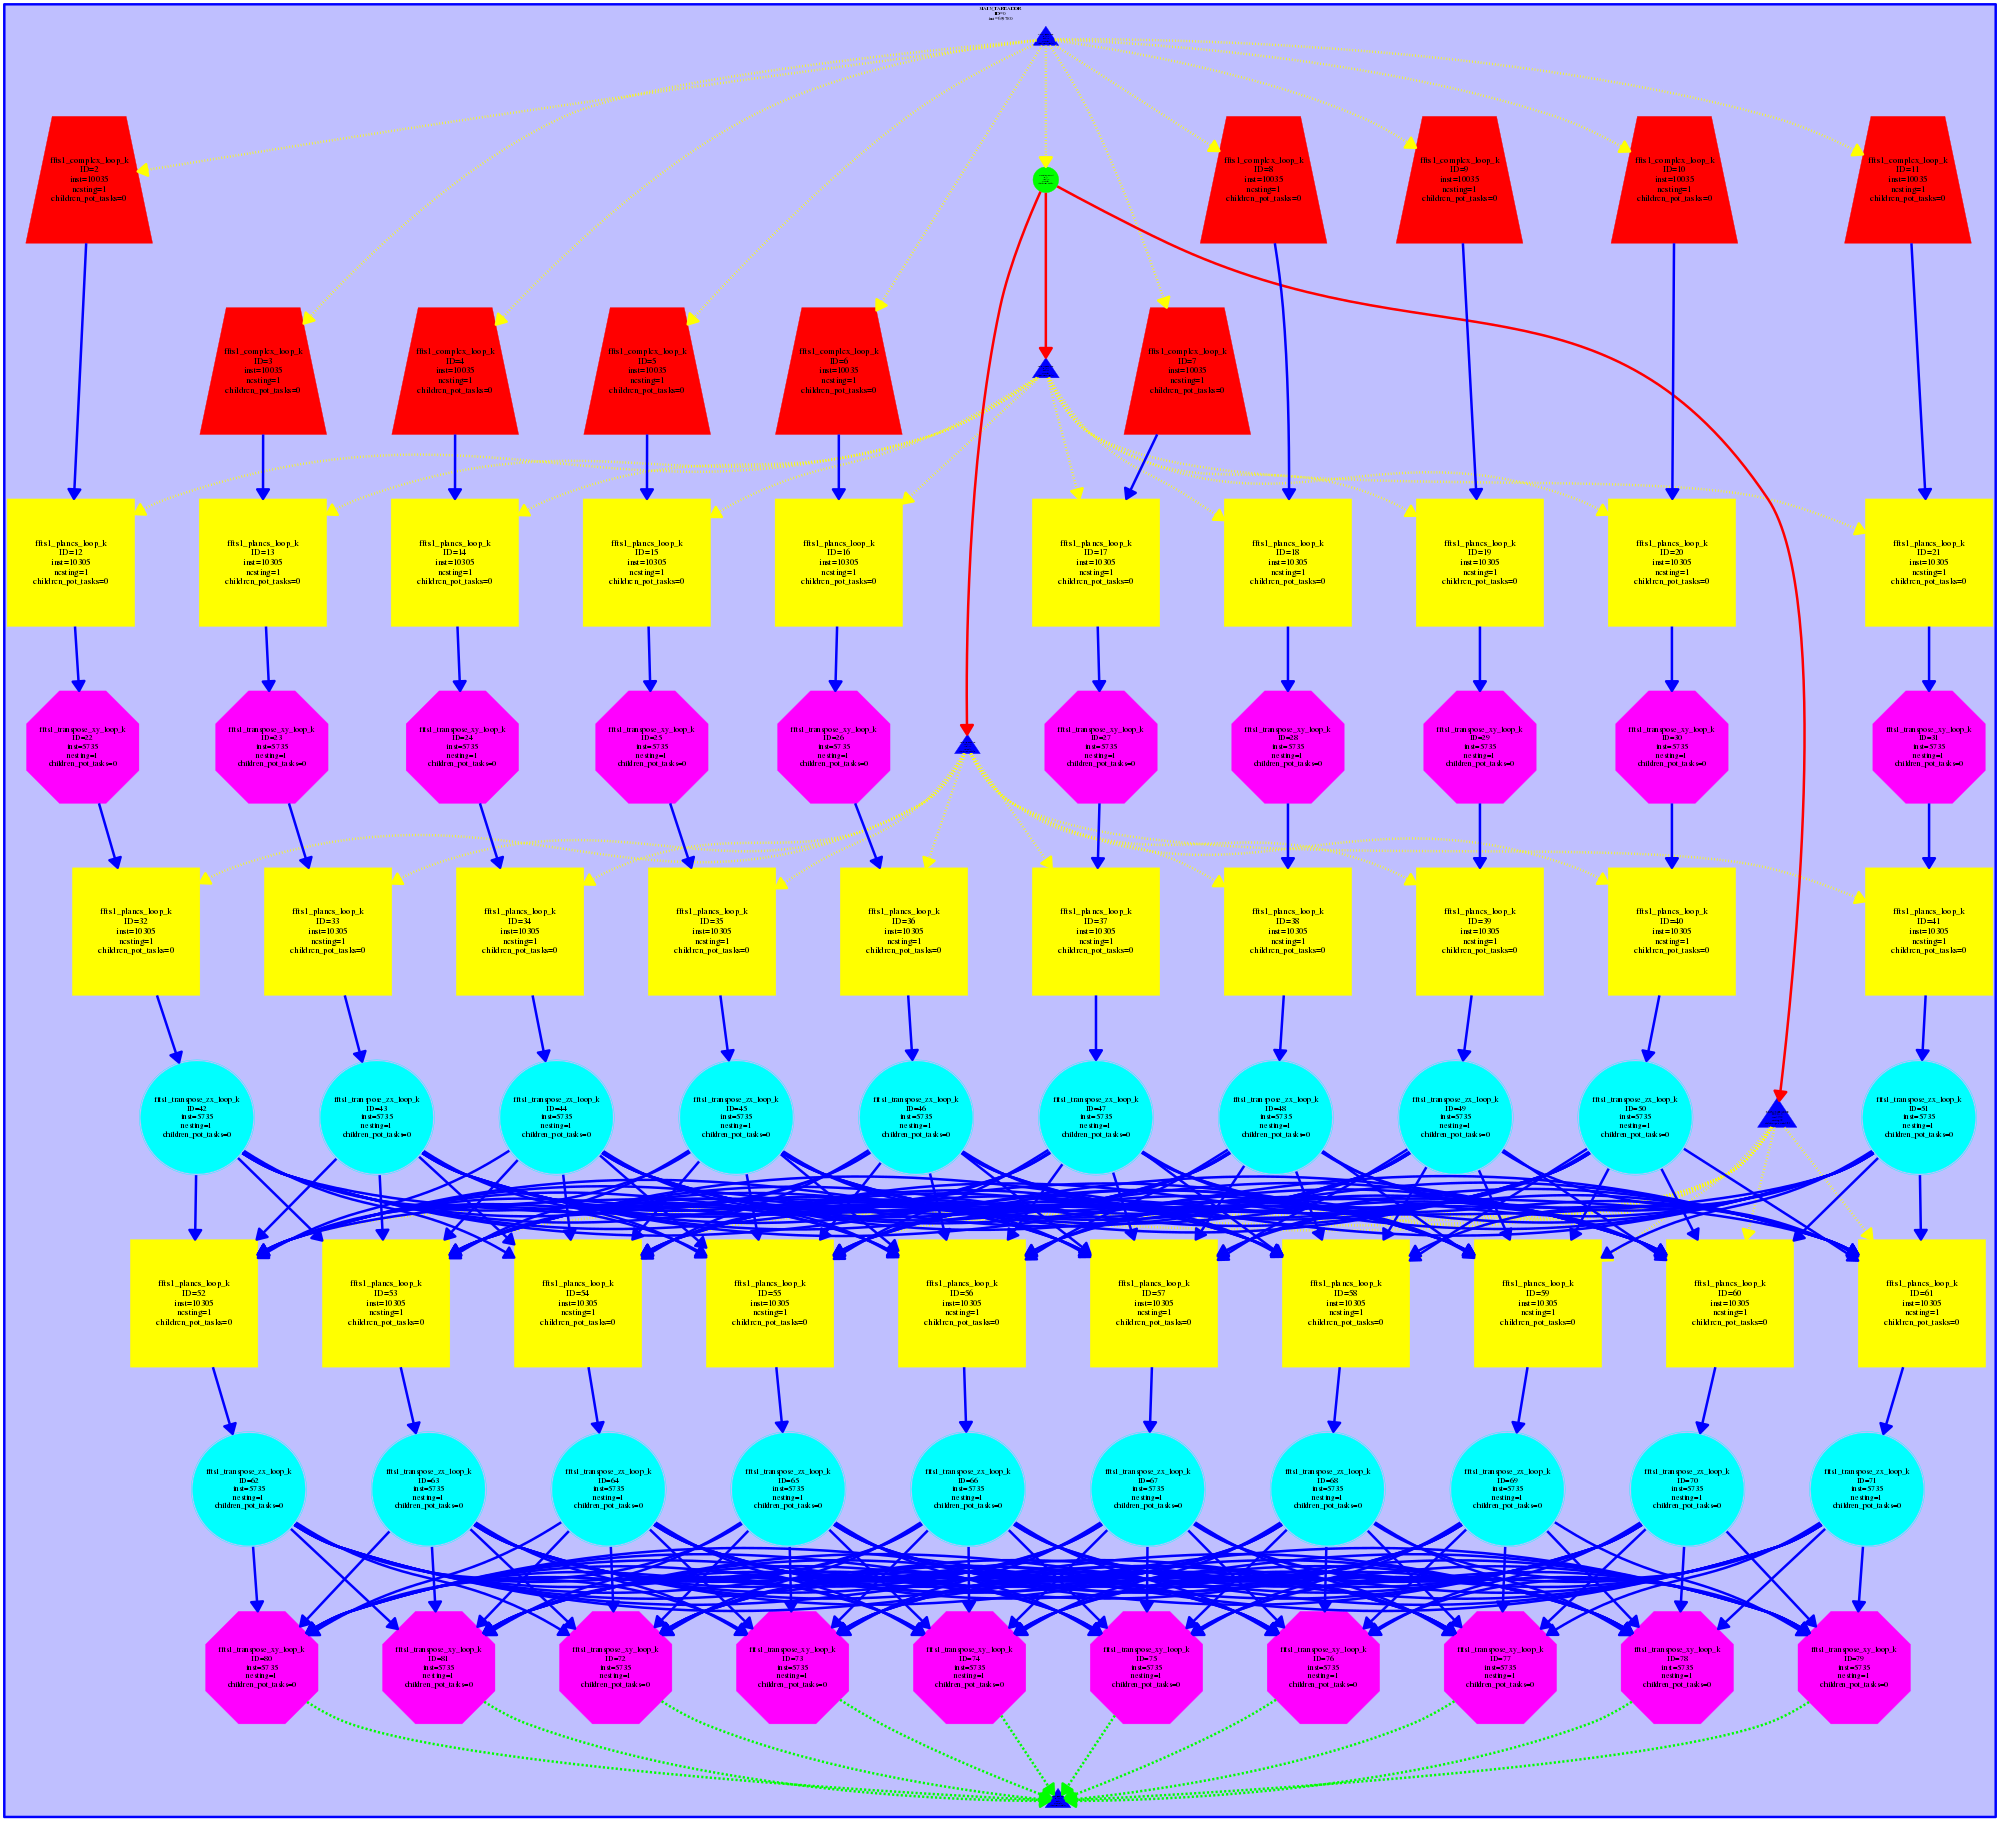
\includegraphics[width=15cm,height=13cm]{./images/dependency_graph_v4}
  \caption{Task dependency graph of version 4.}
  \label{dependency_graph_v4}
\end{figure}

\subsection{Version 5}

Finally, in the last version we had to decompose into smaller tasks the ones that we though that were necessary and useful to decrease T$_\infty$ and increase Parallelism. What we did was to look in the Figure \ref{dependency_graph_v4} the tasks that had a bigger number of instructions. There were 2 functions with the same number of instructions, 10305. These two functions were \textit{init\_complex\_grid} and \textit{ffts1\_planes}.

We "sinked" the creation of the tasks one more loop, so now in \textit{init\_complex\_grid} and \textit{ffts1\_planes} we create $N^2$ tasks, even though in the first one we could have created $N^3$ tasks. We did not that because we though that it could cause a lot of overheads and this was not good.

\[ T_1 = (970 + 20 + 1065 + 1022 + 5735 + 1022 + 5735 + 1022 + 5735 + 5735 + 0) * 1000 \]

\[ = 28061 * 1000 = 28061000 ns \]

\[ Parallelism = T_1/T_\infty = 639780000/28061000 = 22.79961512 \]

In this last version, we got the biggest parallelism of all versions and the smallest critical version. As in version 4, we also had to simulate this version of the code with 1, 2, 4, 8, 16 and 32 processors to analyse the potential strong scalability. This is discussed in the section \ref{Analysis of the potential strong scalability in v4 and v5}.

\begin{lstlisting}
	void init_complex_grid(fftwf_complex in_fftw[][N][N]) {
	  int k,j,i;
	
	  for (k = 0; k < N; k++) {
	    for (j = 0; j < N; j++) {
	      tareador_start_task("ffts1_complex_loop_kj");
	      for (i = 0; i < N; i++)
	      {
	        in_fftw[k][j][i][0] = (float) (sin(M_PI*((float)i)/64.0)+
	        							   sin(M_PI*((float)i)/32.0)+
	        							   sin(M_PI*((float)i/16.0)));
	        in_fftw[k][j][i][1] = 0;
	#if TEST
	        out_fftw[k][j][i][0]= in_fftw[k][j][i][0];
	        out_fftw[k][j][i][1]= in_fftw[k][j][i][1];
	#endif
	      }
	      tareador_end_task("ffts1_complex_loop_kj");
	    }
	  }
	}
	
	void ffts1_planes(fftwf_plan p1d, fftwf_complex in_fftw[][N][N]) {
	    int k,j;
	
	    for (k=0; k<N; k++) {
	     for (j=0; j<N; j++) {
	       tareador_start_task("ffts1_planes_loop_kj");
	         fftwf_execute_dft( p1d, (fftwf_complex *)in_fftw[k][j][0], 
	           			      (fftwf_complex *)in_fftw[k][j][0]);
	       tareador_end_task("ffts1_planes_loop_kj");
	     }
	    }
	}
	
	...
	
	int main() {
	
		...
		
		START_COUNT_TIME;
	
	    tareador_start_task("start_plan_forward");
	    start_plan_forward(in_fftw, &p1d);
	    tareador_end_task("start_plan_forward");
	
	    STOP_COUNT_TIME("3D FFT Plan Generation");
	
	
	    START_COUNT_TIME;
	
	    init_complex_grid(in_fftw);
	
	    STOP_COUNT_TIME("Init Complex Grid FFT3D");
	
	
	    START_COUNT_TIME;
	
	    ffts1_planes(p1d, in_fftw);
	    transpose_xy_planes(tmp_fftw, in_fftw);
	    ffts1_planes(p1d, tmp_fftw);
	    transpose_zx_planes(in_fftw, tmp_fftw);
	    ffts1_planes(p1d, in_fftw);
	    transpose_zx_planes(tmp_fftw, in_fftw);
	    transpose_xy_planes(in_fftw, tmp_fftw);
	     
	    STOP_COUNT_TIME("Execution FFT3D");
	    
	    ...
	}
\end{lstlisting}

\begin{figure}[H]
  \centering
  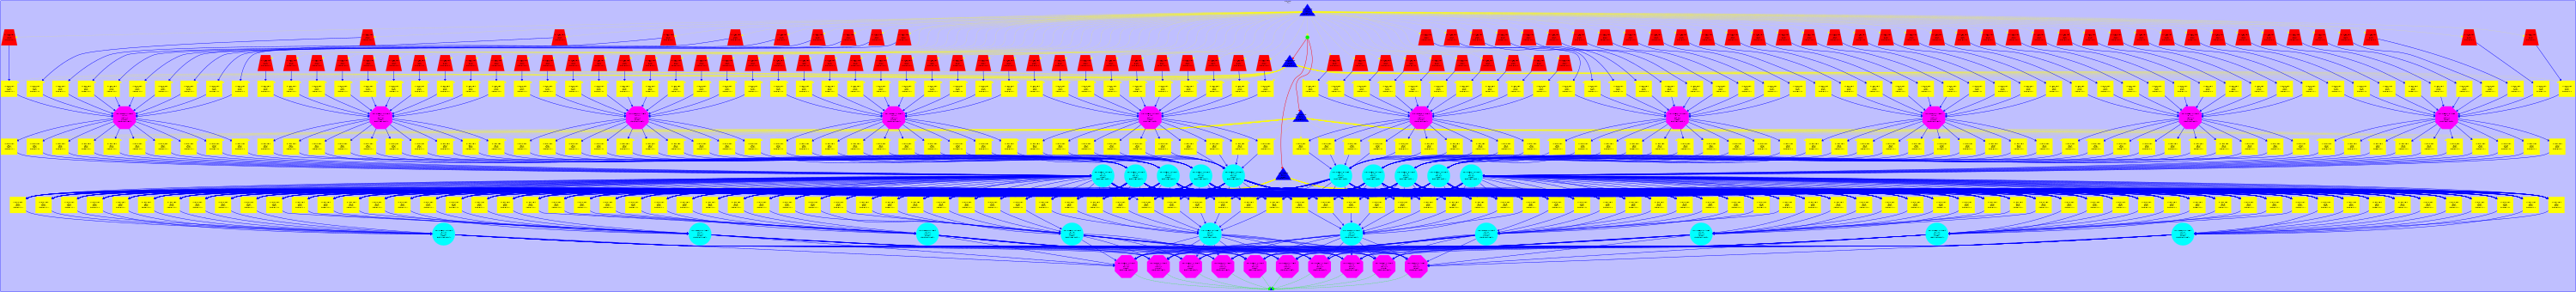
\includegraphics[angle=90, scale=0.20]{./images/dependency_graph_v5}
  \caption{Task dependency graph of version 5.}
  %\label{etiqueta}
\end{figure}

\subsection{Analysis of the potential strong scalability in v4 and v5}

\label{Analysis of the potential strong scalability in v4 and v5}

In v4 and v5 of \textbf{3dfft\_tar.c} we had to analyse the potential strong scalability they had. As we said in the first laboratory session, in \textit{strong} scalability the number of processors is changed with a fixed problem size. In this case parallelism is used to reduce the execution time of the program. We will analyse it using 1, 2, 4, 8, 16 and 32 processors. \textit{Paraver} is very useful in it because it can simulate up to 128 processors and show the T$_p$ of the program. Firstly we will talk about v4 plots and secondly about v5 plots.

As we can see in Figure \ref{fig:texe_v4}, the bigger the number of CPUs, the faster the program runs, achieving a minimum time of execution from 16 processors. This is because the new processors will not execute any instruction. Besides, the Figure \ref{fig:speedup_v4} shows the speedup. Speedup is the relative reduction of execution time when using P processors with respect to sequential (T$_1$/T$_p$). As we said before, we reduced the execution time as we were increasing the number of processors, until 16. For this reason, the speedup increases also until 16 processors.


\begin{figure}[H]
\begin{minipage}[b]{0.45\linewidth}
\centering
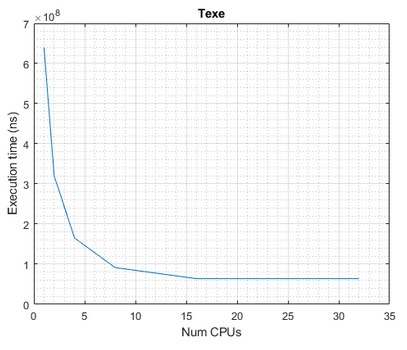
\includegraphics[width=\textwidth]{./images/texe_v4}
\caption{Execution time plot of version 4 as we increase the number of processors.}
\label{fig:texe_v4}
\end{minipage}
\hspace{0.5cm}
\begin{minipage}[b]{0.45\linewidth}
\centering

\begin{center}
\begin{table}
\begin{tabular}{ |c || c| } 
 \hline
 Processors & T$_{exe}$ [ns] \\
 \hline
 \hline 
 1 & 639780001 \\ 
 \hline
 2 & 320310001 \\ 
 \hline
 4 & 165389001 \\ 
 \hline
 8 & 91496001 \\ 
 \hline
 16 & 64018001 \\ 
 \hline
 32 & 64018001 \\ 
 \hline
\end{tabular}
\caption{Values for Figure \ref{fig:texe_v4}.}
\end{table}
\end{center}

\label{fig:figure2}
\end{minipage}
\end{figure}

\begin{figure}[H]
\begin{minipage}[b]{0.45\linewidth}
\centering
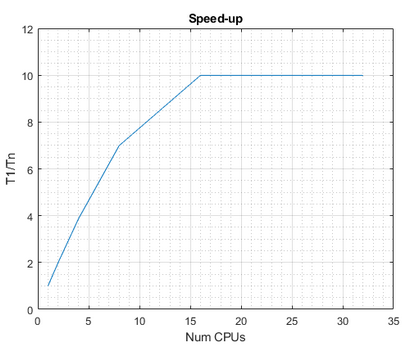
\includegraphics[width=\textwidth]{./images/speedup_v4}
\caption{Speedup plot of version 4 as we increase the number of processors.}
\label{fig:speedup_v4}
\end{minipage}
\hspace{0.5cm}
\begin{minipage}[b]{0.45\linewidth}
\centering

\begin{center}
\begin{table}
\begin{tabular}{ |c || c| } 
 \hline
 Processors & Speed-up \\
 \hline
 \hline 
 1 & 1 \\ 
 \hline
 2 & 1.9973775 \\ 
 \hline
 4 & 3.8683346 \\ 
 \hline
 8 & 6.9924368 \\ 
 \hline
 16 & 9.9937516 \\ 
 \hline
 32 & 9.9937516 \\ 
 \hline
\end{tabular}
\caption{Values for Figure \ref{fig:speedup_v4}.}
\end{table}
\end{center}

\label{fig:figure2}
\end{minipage}
\end{figure}

If we look now in Figures \ref{fig:texe_v5} and \ref{fig:speedup_v5}, we can see very similar plots from the ones explained before. The main difference is that in this two plots, we have not reached a minimum execution time, so simulating the code with more than 32 processors would reduce the time. As a consequence, speedup also has not reached its maximum value, and adding more processors would still increase its value.

\begin{figure}[H]
\begin{minipage}[b]{0.45\linewidth}
\centering
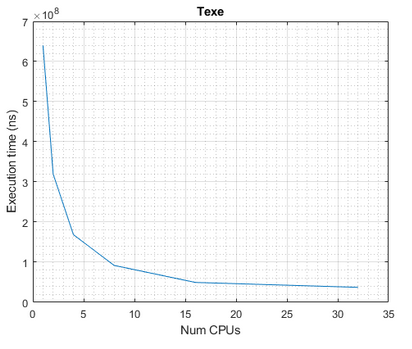
\includegraphics[width=\textwidth]{./images/texe_v5}
\caption{Execution time plot of version 5 as we increase the number of processors.}
\label{fig:texe_v5}
\end{minipage}
\hspace{0.5cm}
\begin{minipage}[b]{0.45\linewidth}
\centering

\begin{center}
\begin{table}
\begin{tabular}{ |c || c| } 
 \hline
 Processors & T$_{exe}$ [ns] \\
 \hline
 \hline 
 1 & 639780001 \\ 
 \hline
 2 & 320020001 \\ 
 \hline
 4 & 168343001 \\ 
 \hline
 8 & 92001001 \\ 
 \hline
 16 & 49520001 \\ 
 \hline
 32 & 37337001 \\ 
 \hline
\end{tabular}
\caption{Values for Figure \ref{fig:texe_v5}.}
\end{table}
\end{center}

\label{fig:figure2}
\end{minipage}
\end{figure}



\begin{figure}[H]
\begin{minipage}[b]{0.45\linewidth}
\centering
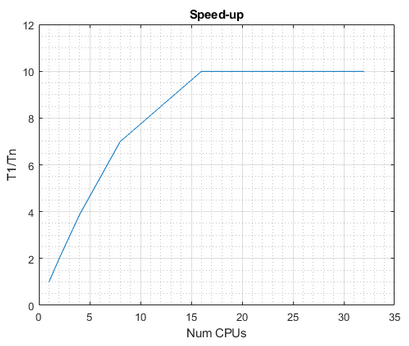
\includegraphics[width=\textwidth]{./images/speedup_v5}
\caption{Speedup plot of version 5 as we increase the number of processors.}
\label{fig:speedup_v5}
\end{minipage}
\hspace{0.5cm}
\begin{minipage}[b]{0.45\linewidth}
\centering

\begin{center}
\begin{table}
\begin{tabular}{ |c || c| } 
 \hline
 Processors & Speed-up \\
 \hline
 \hline 
 1 & 1 \\ 
 \hline
 2 & 1.9991875 \\ 
 \hline
 4 & 3.8004550 \\ 
 \hline
 8 & 6.9540548 \\ 
 \hline
 16 & 12.919628 \\ 
 \hline
 32 & 17.135281 \\ 
 \hline
\end{tabular}
\caption{Values for Figure \ref{fig:speedup_v5}.}
\end{table}
\end{center}

\label{fig:figure2}
\end{minipage}
\end{figure}


Figures \ref{fig:v4_code} and \ref{fig:v5_code} show the main differences of the code between v4 and v5. These are "compact" codes. For more information see the codes of the sections Version 4 and Version 5.

We could easily see that in Figure \ref{dependency_graph_v4} tasks \textit{ffts1\_complex\_loop\_k} and \textit{ffts1\_planes\_loop\_k} were the ones with more number of instructions, so these were the ones we had to decompose into finer\textendash gained tasks. For this reason, in \textit{init\_complex\_grid} function the tasks are now created inside the second loop unlike v4, that were created within the first loop. We could have created smaller tasks if we had created the tasks inside the most inner loop.

On the other hand, in \textit{ffts1\_planes} function we now create the tasks inside the second loop.

These two changes have increased a lot the parallelism.

\begin{figure}[H]
\begin{minipage}[b]{0.55\linewidth}

\begin{lstlisting}
void init_complex_grid(...) {
  int k,j,i;

  for (k = 0; k < N; k++) {
    tareador_start_task("v4_complex");
    for (j = 0; j < N; j++) {
      for (i = 0; i < N; i++)
      {
        ...
      }
    }
    tareador_end_task("v4_complex");
  }
}

void ffts1_planes(...) {
    int k,j;

    for (k=0; k<N; k++) {
     tareador_start_task("v4_planes");
     for (j=0; j<N; j++) {
       ...
     }
     tareador_end_task("v4_planes");
    }
}
\end{lstlisting}

\caption{Compact code of version 4.}
\label{fig:v4_code}
\end{minipage}
\hspace{0.5cm}
\begin{minipage}[b]{0.57\linewidth}

\begin{lstlisting}
void init_complex_grid(...) {
  int k,j,i;

  for (k = 0; k < N; k++) {
    for (j = 0; j < N; j++) {
      tareador_start_task("v5_complex");
      for (i = 0; i < N; i++)
      {
        ...
      }
      tareador_end_task("v5_complex");
    }
  }
}

void ffts1_planes(...) {
    int k,j;

    for (k=0; k<N; k++) {
     for (j=0; j<N; j++) {
       tareador_start_task("v5_planes");
           ...
       tareador_end_task("v5_planes");
     }
    }
}
\end{lstlisting}

\caption{Compact code of version 5.}
\label{fig:v5_code}
\end{minipage}
\end{figure}

\subsection{Summary Table}

To conclude with this section, table \ref{T1, Tinfty and parallelism} summarizes all the information extracted from \textit{Tareador}, \textit{Paraver} and the manual calculations.

T$_1$ using \textit{Tareador} was calculated simulating the execution with 1 processor and T$_\infty$ simulating the execution with the maximum number of processors that \textit{Paraver} can, 128.

\begin{center}
 \begin{table}
 \begin{tabular}{|c || c | c | c | c|} 
 \hline
 
    \multicolumn{2}{|c|}{\textbf{Version}} & T$_1$ [ns] & T$_\infty$ [ns] & \textbf{Parallelism}\\\hline\hline
    \multirow{2}{*}{\textbf{seq}} & \textbf{Manual} & 639780000 & 639760000 & 1.000031262 \\\cline{2-5}
    & \textbf{Tareador} & 639780001 & 639760001 & 1.000031262\\
    
 \hline
 
    \multirow{2}{*}{\textbf{v1}} & \textbf{Manual} & 639780000 & 639760000 & 1.000031262\\\cline{2-5}
    & \textbf{Tareador} & 639780001 & 639707001 & 1.000114115\\
    
 \hline
 
    \multirow{2}{*}{\textbf{v2}} & \textbf{Manual} & 639780000 & 361190000 & 1.771311498\\\cline{2-5}
    & \textbf{Tareador} & 639780001 & 361190001 & 1.771311496\\
  
 \hline
  
    \multirow{2}{*}{\textbf{v3}} & \textbf{Manual} & 639780000 & 154354000 & 4.144887726\\\cline{2-5}
    & \textbf{Tareador} & 639780001 & 154354001 & 4.144887705\\
  
 \hline
  
    \multirow{2}{*}{\textbf{v4}} & \textbf{Manual} & 639780000 & 64018001 & 9.993751601\\\cline{2-5}
    & \textbf{Tareador} & 639780001 & 64018001 & 9.993751601\\
  
 \hline
  
    \multirow{2}{*}{\textbf{v5}} & \textbf{Manual} & 639780000 & 28061000 & 22.79961512\\\cline{2-5}
    & \textbf{Tareador} & 639780001 & 27971001 & 22.87297480\\
  
 \hline
 
 
 
 \hline
\end{tabular}

 \caption{Analysis of task decompositions for the 3dfft program.}
 \label{T1, Tinfty and parallelism}
\end{table}
\end{center}


\section{Understanding the parallel execution of 3DFFT}

In this final session, we had to work with the \textit{Paraver} environment, used to gather information about the execution of a parallel application in \textit{OpenMP} and visualize it.

We had to calculate several things:

\begin{itemize}
	\item T$_1$: This is the execution time using only 1 processor (sequential). We can get this value from the \textit{Paraver}.
	\item T$_8$: This is the execution time using 8 processors at the same time. This value can also be extracted from \textit{Paraver}, simulating the code with 8 CPUs.
	\item S$_8$: The speedup we have using 8 processors. We can obtain this value dividing T$_1$ by T$_8$.
	\item $\phi$: Represents the amount of parallelised code with respect to the total.
	\item S$_\infty$: Speedup we would get if we had an infinite number of processors. To get this value, we had to compute the following equation: $T_{par}/(T_{seq} + T_{par})$.
\end{itemize}

All these data can be found in \textit{Paraver} or computed by ourselves. In this case, we are not going to use 8 processors but 8 threads.

\subsection{Initial version}

In this part, we started finding the T\textsubscript{par} of the execution with one thread using the \textit{OMP\_parallel\_functions\_duration} configuration and the \textit{OMP\_state\_profile}. These two configurations helped us on it. Then, we just had to sum all the execution times of the diferent parallelised functions. The results are the following:

\[T_{par} = 1535434.96 us = 1535434960 ns \] 

Afterwards, we wanted to find the sequential time of the program. To do this, we got the total time of the program with one thread. In Figure \ref{v0_t1} we can see the trace using only 1 thread. In the lower right corner we can find the total execution time (T$_1$). Figure \ref{v0_excel_t1} shows the same information but in a table. Summing all the values of the "Total" row will result in the same value than the Figure \ref{v0_t1}.

\[T_1 = 2378316048 ns \]

\begin{figure}[H]
  \centering
  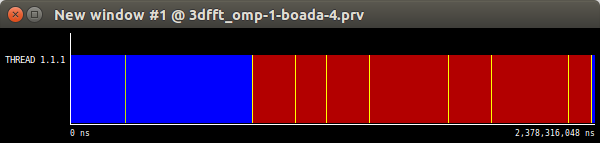
\includegraphics[scale=0.5]{./images/v0_t1}
  \caption{Trace of the execution with 1 thread.}
  \label{v0_t1}
\end{figure}

\begin{figure}[H]
  \centering
  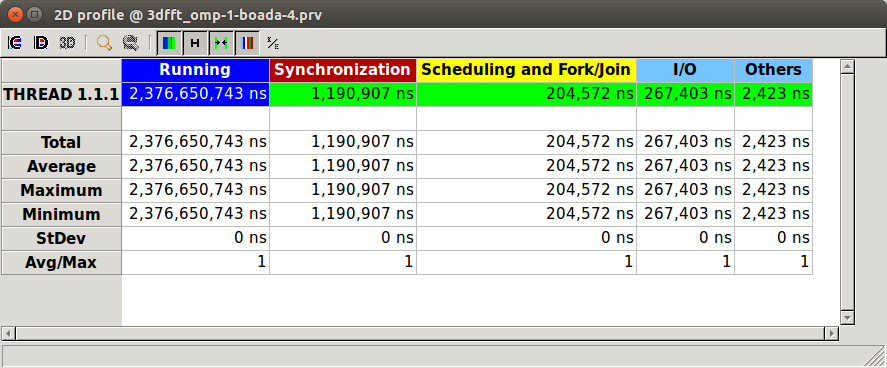
\includegraphics[scale=0.5]{./images/v0_excel_t1}
  \caption{Table of the diferent states that thread 1 has been.}
  \label{v0_excel_t1}
\end{figure}

 Then, applying the following formulas, we could find T$_{seq}$ and $\phi$.

\[T_{seq} = T_1 - T_{par} = 2378316048 - 1535434.96 * 1000 = 842881088 ns \]

\[\phi = \dfrac{T_{par}} {T_{seq} + T_{par}} = \dfrac{1535434960} {842881088 + 1535434960} = 0.64559752741 \]
\[\phi = 64.559752741\%\]

Then we have changed the trace for the one that has been processed with 8 threads. Figure \ref{v0_t8} shows the execution time with 8 threads and the work that each one does.

\[T_{8} = 1609711162 ns \]

\begin{figure}[H]
  \centering
  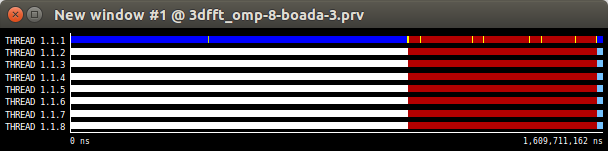
\includegraphics[scale=0.5]{./images/v0_t8}
  \caption{Trace of the execution with 8 threads.}
  \label{v0_t8}
\end{figure}

Then, we had to compute S$_8$. We calculated this as following:

\[ S_{8} = \dfrac{T_{1}}{T_{8}} = \dfrac{2378316048} {1609711162} = 1.47748000023 \]

Before calculating S$_\infty$, we had to compute again T$_1$, T$_8$ and S$_8$, but with a different script. This is because \textit{Paraver} is introducing some extra time needed to initialise the instrumentation, but then the behaviour is reflected accurately with no much overhead. Now, executing the script \textbf{submit-omp.sh} will not produce this "extra time". We got 3 different values, corresponding to the different parallelised parts: 3D FFT Plan Generation, Init Complex Grid and Execution FFT3D. Summing up all these 3 values will result in T$_1$ and T$_8$ depending on the number of processors executing the code.

\[T_1 = 0.005400 + 0.577763 + 1.737352 = 2.320515 s = 2320515000 ns \]

\[T_8 = 0.000551 + 0.576197 + 0.559041 = 1.135789 s = 1135789000 ns \]

\[S_8 = \dfrac{T_1}{T_8} = \dfrac{2320515000}{1135789000} = 2.0430863479 \]

We can observe that there is a big overhead when using \textit{Paraver}. If we do not use it, we increase the speedup a lot. Finally we can compute the S$_\infty$ using the next equation:

\[S_\infty = \dfrac{1}{1 - \phi} = \dfrac{1} {1 - 0.64559752741} = 2.8216507427 \]

This means that with a 64.55 \% of the code parallelised, we will only be able to execute the program 2.82 times faster. The following figures show the evolution of the execution time and the speedup as we increase the number of threads (strong scalability).

\begin{figure}[H]
\begin{minipage}[b]{0.45\linewidth}
\centering
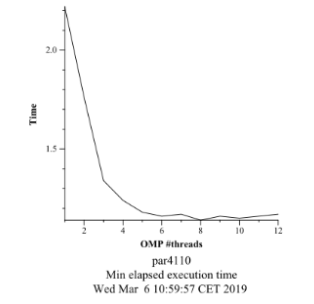
\includegraphics[width=\textwidth]{./images/min_v0}
\caption{Execution time plot as we increase the number of threads.}
\label{fig:min_v0}
\end{minipage}
\hspace{0.5cm}
\begin{minipage}[b]{0.45\linewidth}
\centering
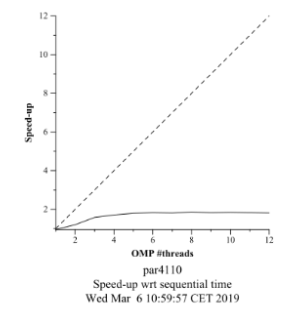
\includegraphics[width=\textwidth]{./images/speed_v0}

\caption{Speedup plot as we increase the number of threads.}
\label{fig:speed_v0}
\end{minipage}
\end{figure}

\subsection{Improving $\phi$}

In this part of the laboratory, we had to find the part of the code that make our code to be less parallelized. This part was the function init\_complex\_grid. To increase the parallelism we uncommented the pragma shown in the next code.

\begin{lstlisting}
void init_complex_grid(fftwf_complex in_fftw[][N][N]) {

  #pragma omp parallel
	for (int k = 0; k < N; k++) 
		#pragma omp for schedule(static, 1)
    for (int j = 0; j < N; j++)
      for (int i = 0; i < N; i++)
      {
				in_fftw[k][j][i][0] = (float) (sin(M_PI*((float)i)/64.0)
									+ sin(M_PI*((float)i)/32.0)
									+ sin(M_PI*((float)i/16.0)));
        in_fftw[k][j][i][1] = 0;
#if TEST
        out_fftw[k][j][i][0]= in_fftw[k][j][i][0];
        out_fftw[k][j][i][1]= in_fftw[k][j][i][1];
#endif
      }
}
\end{lstlisting}

Now we had to compute the same equations that we applied in the 1st part in order to find the results for the table. T$_1$ has not exactly the same value than the previous section. We think that \textit{Paraver} is the culprit.

\[T_1 = 2377989045 ns \] 
\[T_{par} = 2066229470 ns \]
\[T_{seq} = 2377989045 - 2066229470 = 311759575 ns \]
\[\phi = \dfrac{T_{par}} {T_{seq} + T_{par}} = \dfrac{2066229470} {311759575 + 2066229470} = 0.86889780856 \]
\[\phi = 86.889780856\% \]

\[T_8 = 887257925 ns \]
\[S_8 = \dfrac{T_1}{T_8} = \dfrac{2377989045}{887257925} = 2.68015531673 \]
\[S_\infty = \dfrac{1}{1 - \phi} = \dfrac{1} {1 - 0.86889780856} = 7.62763756285 \]

It makes sense that all the speedup values have increased and the execution times have decreased, because as we have augmented the parallelism, more threads can now execute code at the same time. Some of the previous values have been extracted from the following figures:

\begin{figure}[H]
  \centering
  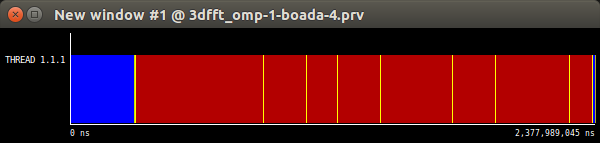
\includegraphics[scale=0.5]{./images/v1_t1}
  \caption{Trace of the execution with 1 thread.}
  \label{v1_t1}
\end{figure}

\begin{figure}[H]
  \centering
  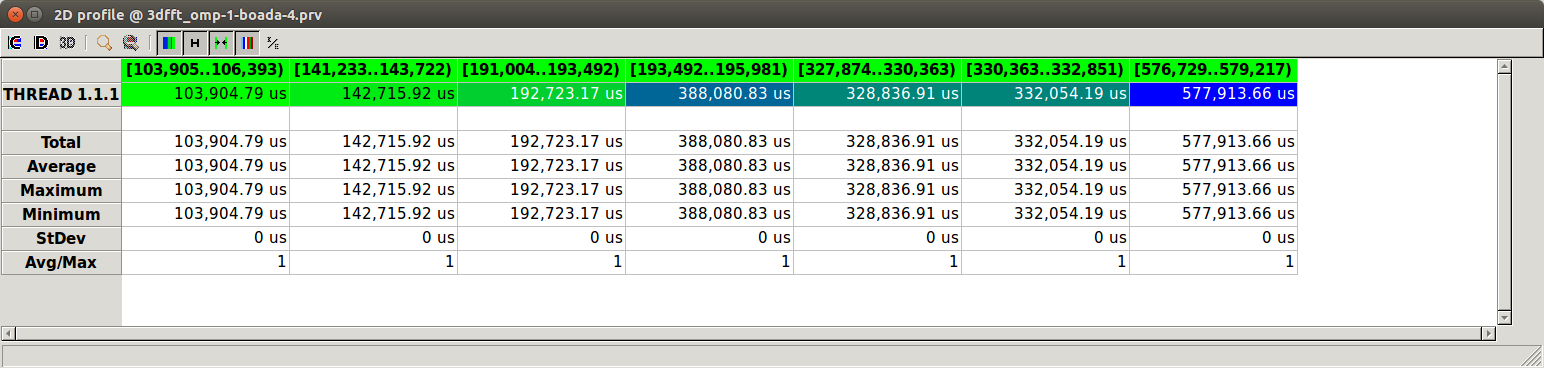
\includegraphics[scale=0.25]{./images/v1_excel_tpar}
  \caption{Table of the times of the different parallelised functions.}
  \label{v1_excel_tpar}
\end{figure}

\begin{figure}[H]
  \centering
  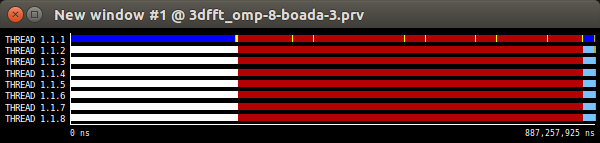
\includegraphics[scale=0.5]{./images/v1_t8}
  \caption{Trace of the execution with 8 threads.}
  \label{v1_t8}
\end{figure}

Finally, in figures \ref{fig:min_v1} and \ref{fig:speed_v1} we can see that the speedup increases more than the figure of the previous section and the time starts to increase again when the number of threads is equal to 10 (in the previous section it started in 8 threads).

\begin{figure}[H]
\begin{minipage}[b]{0.45\linewidth}
\centering
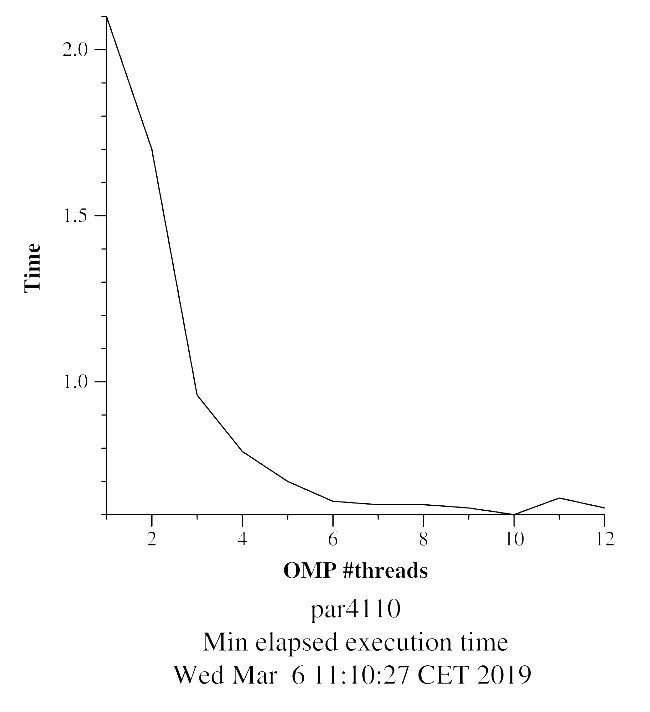
\includegraphics[width=\textwidth]{./images/min_v2}
\caption{Execution time plot as we increase the number of threads.}
\label{fig:min_v1}
\end{minipage}
\hspace{0.5cm}
\begin{minipage}[b]{0.45\linewidth}
\centering
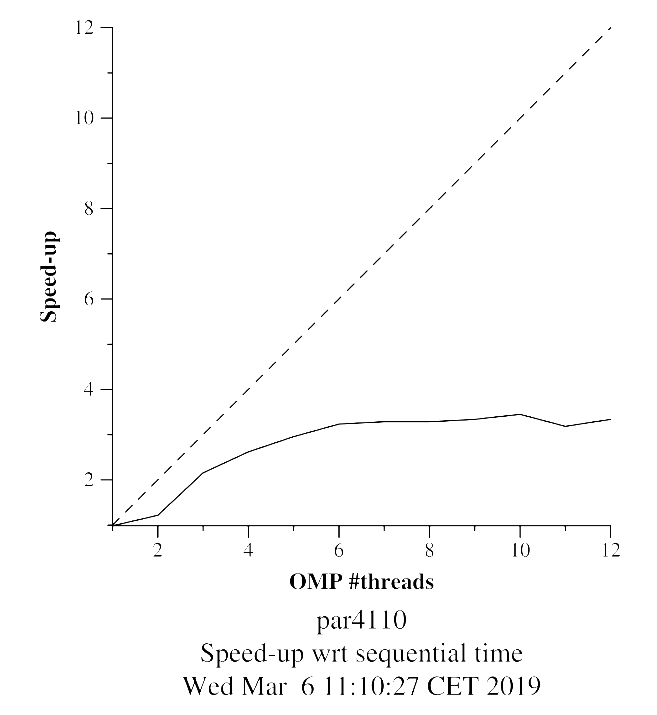
\includegraphics[width=\textwidth]{./images/speed_v2}

\caption{Speedup plot as we increase the number of threads.}
\label{fig:speed_v1}
\end{minipage}
\end{figure}

\subsection{Reducing parallelisation overheads}

Lastly, we had to increase the granularity of tasks by moving one line up the second pragma of each function. For example:

\begin{lstlisting}
	void init_complex_grid(fftwf_complex in_fftw[][N][N]) {
	
		#pragma omp parallel
		#pragma omp for schedule(static, 1)
		for (int k = 0; k < N; k++) 
			for (int j = 0; j < N; j++)
				for (int i = 0; i < N; i++)
				{
					in_fftw[k][j][i][0] = (float) (sin(M_PI*((float)i)/64.0)
										+ sin(M_PI*((float)i)/32.0)
										+ sin(M_PI*((float)i/16.0)));
					in_fftw[k][j][i][1] = 0;
	#if TEST
					out_fftw[k][j][i][0]= in_fftw[k][j][i][0];
					out_fftw[k][j][i][1]= in_fftw[k][j][i][1];
	#endif
				}
	}
\end{lstlisting}

This change allowed us to reduce the parallization overheads getting a better performance as seen in the following equations (the same that are explained in the 1st part).

\[T_1 = 2349744097 ns \]
\[T_{par} = 2081319010 ns \]
\[T_{seq} = 2349744097 - 2081319010 = 268425087 ns \]
\[\phi = \dfrac{T_{par}} {T_{seq} + T_{par}} = \dfrac{2081319010} {268425087 + 2081319010} = 0.88576411901 \]
\[\phi = 88.576411901\% \]

\[T_8 = 639450975 ns \]
\[S_8 = \dfrac{T_1}{T_8} = \dfrac{2349744097}{639450975} = 3.67462743645 \]
\[S_\infty = \dfrac{1}{1 - \phi} = \dfrac{1} {1 - 0.88576411901} = 8.75381702608 \]

We can see that this change made us to improve the S$_8$ (2.68 to 3.67) and S$_\infty$ (7.62 to 8.75). Following we show some of the traces and tables we have used to compute all these values.

\begin{figure}[H]
  \centering
  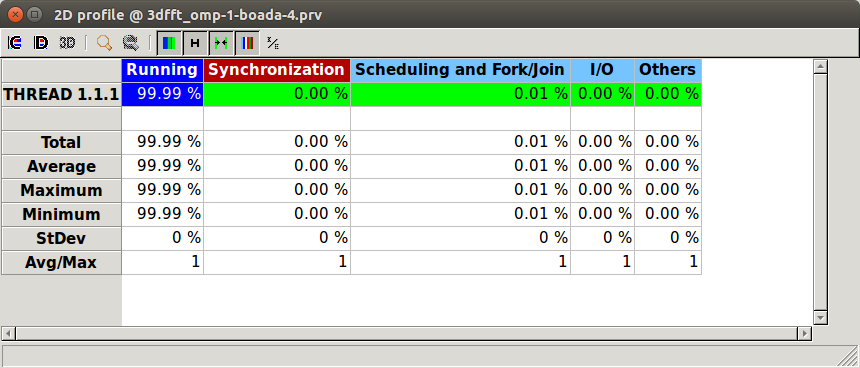
\includegraphics[scale=0.5]{./images/v2_t1}
  \caption{Table of the diferent states that thread 1 has been.}
  \label{v2_t1}
\end{figure}

\begin{figure}[H]
  \centering
  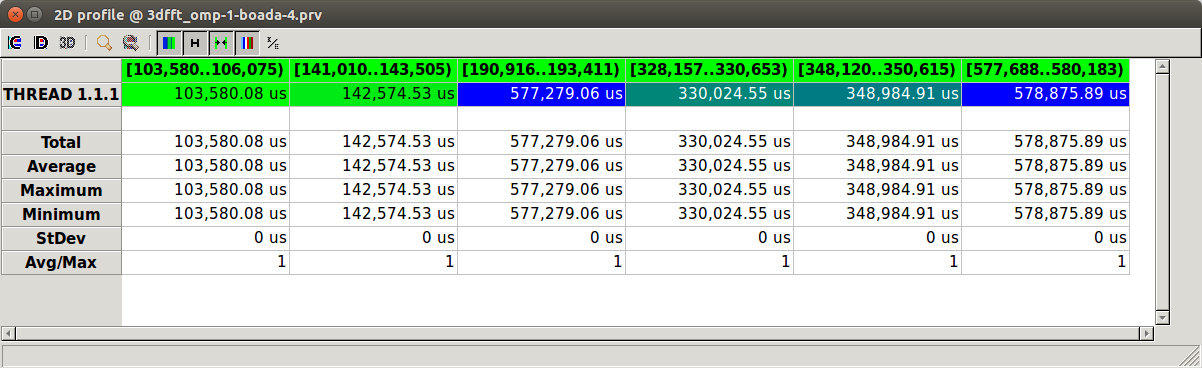
\includegraphics[scale=0.35]{./images/v2_tpar}
  \caption{Table of the times of the different parallelised functions.}
  \label{v2_tpar}
\end{figure}

\begin{figure}[H]
  \centering
  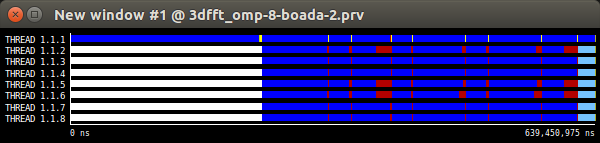
\includegraphics[scale=0.5]{./images/v2_t8}
  \caption{Trace of the execution with 8 threads.}
  \label{v2_t8}
\end{figure}

Figures \ref{fig:min_v2} and \ref{fig:speed_v2} show the improvement we achieved. The speedup is the biggest between the three codes and the time still decreases when we have 10 threads.

\begin{figure}[H]
\begin{minipage}[b]{0.45\linewidth}
\centering
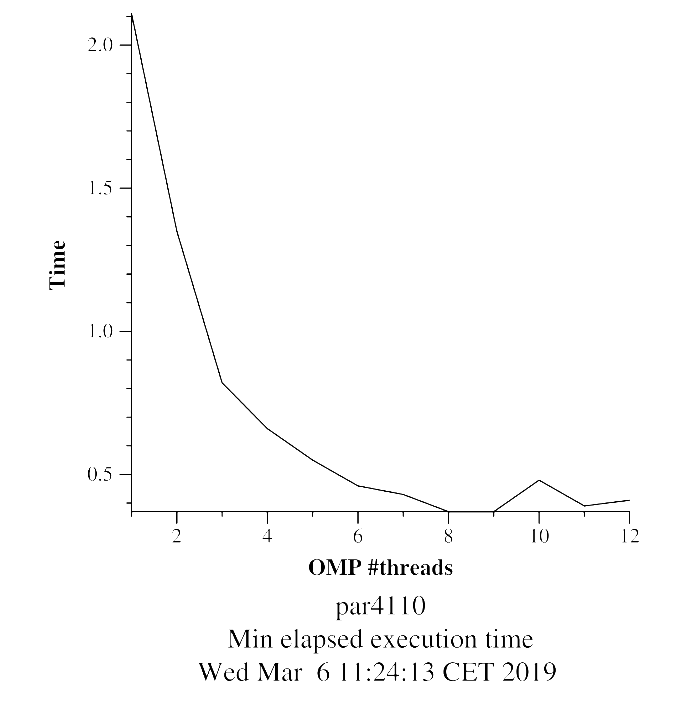
\includegraphics[width=\textwidth]{./images/min_v1}
\caption{Execution time plot as we increase the number of threads.}
\label{fig:min_v2}
\end{minipage}
\hspace{0.5cm}
\begin{minipage}[b]{0.45\linewidth}
\centering
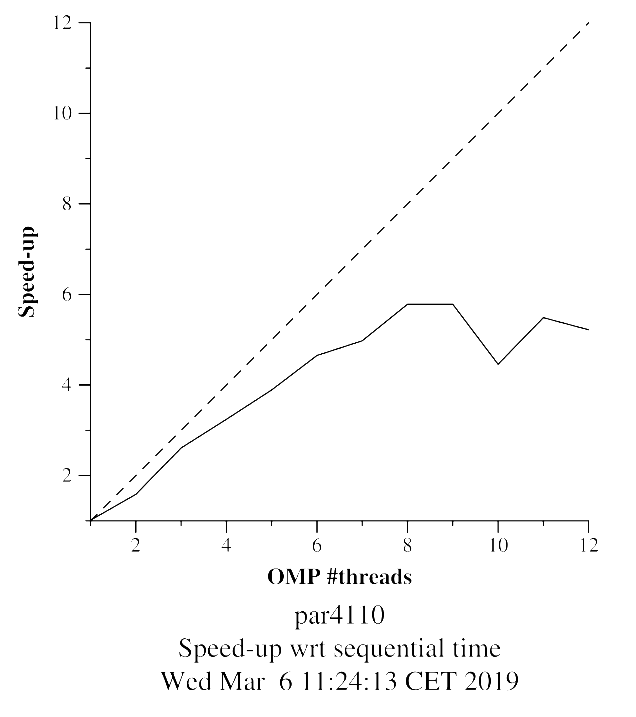
\includegraphics[width=\textwidth]{./images/speed_v1}

\caption{Speedup execution time plot as we increase the number of threads.}
\label{fig:speed_v2}
\end{minipage}
\end{figure}


\subsection{Conclusions}
\begin{center}
	\begin{table}
 \begin{tabular}{|c || c | c || c | c | c|} 
 \hline
 \textbf{Version} & $\phi$ (\%) & S$_\infty$ & T$_1$ (s) & T$_8$ (s) & S$_8$ \\
 \hline\hline
 initial version in \textbf{3dfft\_omp.c} & 64.55 & 2.82 & 2.38 & 1.61 & 1.48 \\ 
 \hline
 new version with improved $\phi$ & 86.89 & 7.63 & 2.38 & 0.89 & 2.68 \\
 \hline
 final version with reduced parallelisation overheads & 88.58 & 8.75 & 2.35 & 0.64 & 3.67 \\
 \hline
\end{tabular}
\caption{Analysis of execution time of 3dfft program.}
\label{Texe}
\end{table}
\end{center}

In this code, we have been able to observe the temporary improvement in the evolution of the code. First of all, when we added parallelism in the first function there has been a great change especially in the scalability, since much of the sequential code has been part of the parallel. Next, by increasing the granularity of the tasks, we have seen a small improvement, especially in the parallel part, since we have been able to reduce overheads. 

\end{document}
